%%%%%%%%%%%%%%%%%%%%%%%%%%%%%%%%%%%%%%%%%%%%%%
%%%%%%%%%%%%%%%%%%%%%%%%%%%%%%%%%%%%%%%%%%%%%%
%%                                          %%
%% Important note on usage                  %%
%% -----------------------                  %%
%% This file must be compiled with PDFLaTeX %%
%% Using standard LaTeX will not work!      %%
%%                                          %%
%%%%%%%%%%%%%%%%%%%%%%%%%%%%%%%%%%%%%%%%%%%%%%
%%%%%%%%%%%%%%%%%%%%%%%%%%%%%%%%%%%%%%%%%%%%%%

%% The '3p' and 'times' class options of elsarticle are used for Elsevier CRC
% \documentclass[5p]{elsarticle}
% Good for final formatting  - two column
% 
% \documentclass[3p,times]{elsarticle}
\documentclass[3p]{elsarticle}
% Good for proofing - single column
% 

\usepackage[american]{babel}
\usepackage{amsmath}
\usepackage[version=3]{mhchem} 
% \usepackage{fixltx2e}
% \usepackage{refcount}
% \usepackage{siunitx}
% \usepackage{lastpage}
% \usepackage{textcomp}
\usepackage{mathtools}

\usepackage{xfrac}
\usepackage{lmodern}
\usepackage[hidelinks]{hyperref}
% \usepackage{cool}
% \usepackage{cancel}
\usepackage{microtype}
\usepackage{listings}
\usepackage{mcode}
\usepackage [autostyle, english = american]{csquotes}
\usepackage{longtable}
\usepackage{subcaption}
\usepackage{booktabs,siunitx}
\usepackage{gensymb}
\usepackage[normalem]{ulem}

% \usepackage{mathtools, cuted}


% \usepackage[usenames,dvipsnames,svgnames,table]{xcolor}
\usepackage{color}

\usepackage[colorinlistoftodos]{todonotes}

\usepackage[section]{placeins}
\usepackage{multirow}

\usepackage{lineno}



\lstset{basicstyle=\small\ttfamily,columns=fullflexible}

% \usepackage{verbatim}



% \usepackage{gensymb}
% \usepackage{enumerate}
% \usepackage{float}
% \usepackage{bm}
% \usepackage{csquotes}
% \usepackage{mathtools}
\usepackage{natbib}
% \usepackage{biblatex}

%% The `ecrc' package must be called to make the CRC functionality available
\usepackage{ecrc}

%% The ecrc package defines commands needed for running heads and logos.
%% For running heads, you can set the journal name, the volume, the starting page and the authors

%% set the volume if you know. Otherwise `00'
\volume{00}

%% set the starting page if not 1
\firstpage{1}

%% Give the name of the journal
\journalname{Nuclear Instruments and Methods in Physics Research B}

%% Give the author list to appear in the running head
%% Example \runauth{C.V. Radhakrishnan et al.}
\runauth{A.S. Voyles et al.}

%% The choice of journal logo is determined by the \jid and \jnltitlelogo commands.
%% A user-supplied logo with the name <\jid>logo.pdf will be inserted if present.
%% e.g. if \jid{yspmi} the system will look for a file yspmilogo.pdf
%% Otherwise the content of \jnltitlelogo will be set between horizontal lines as a default logo

%% Give the abbreviation of the Journal.
\jid{nimb}
% \jid{yspmi}

%% Give a short journal name for the dummy logo (if needed)
\jnltitlelogo{Nucl Instrum Meth B}

%% Hereafter the template follows `elsarticle'.
%% For more details see the existing template files elsarticle-template-harv.tex and elsarticle-template-num.tex.

%% Elsevier CRC generally uses a numbered reference style
%% For this, the conventions of elsarticle-template-num.tex should be followed (included below)
%% If using BibTeX, use the style file elsarticle-num.bst

%% End of ecrc-specific commands
%%%%%%%%%%%%%%%%%%%%%%%%%%%%%%%%%%%%%%%%%%%%%%%%%%%%%%%%%%%%%%%%%%%%%%%%%%

%% The amssymb package provides various useful mathematical symbols
\usepackage{amssymb}
%% The amsthm package provides extended theorem environments
\usepackage{amsthm}

%% The lineno packages adds line numbers. Start line numbering with
%% \begin{linenumbers}, end it with \end{linenumbers}. Or switch it on
%% for the whole article with \linenumbers after \end{frontmatter}.
%% \usepackage{lineno}

%% natbib.sty is loaded by default. However, natbib options can be
%% provided with \biboptions{...} command. Following options are
%% valid:

%%   round  -  round parentheses are used (default)
%%   square -  square brackets are used   [option]
%%   curly  -  curly braces are used      {option}
%%   angle  -  angle brackets are used    <option>
%%   semicolon  -  multiple citations separated by semi-colon
%%   colon  - same as semicolon, an earlier confusion
%%   comma  -  separated by comma
%%   numbers-  selects numerical citations
%%   super  -  numerical citations as superscripts
%%   sort   -  sorts multiple citations according to order in ref. list
%%   sort&compress   -  like sort, but also compresses numerical citations
%%   compress - compresses without sorting
%%
%% \biboptions{comma,round}

\biboptions{sort&compress}

% if you have landscape tables
\usepackage[figuresright]{rotating}

% put your own definitions here:
%   \newcommand{\cZ}{\cal{Z}}
%   \newtheorem{def}{Definition}[section]
%   ...

% add words to TeX's hyphenation exception list
%\hyphenation{author another created financial paper re-commend-ed Post-Script}

% declarations for front matter

\usepackage{fancyvrb}
\usepackage{color}
 
\definecolor{mygreen}{rgb}{0,0.6,0}
\definecolor{mygray}{rgb}{0.5,0.5,0.5}
\definecolor{mymauve}{rgb}{0.58,0,0.82}

\lstset{ %
  backgroundcolor=\color{white},   % choose the background color
  basicstyle=\footnotesize,        % size of fonts used for the code
  breaklines=true,                 % automatic line breaking only at whitespace
  captionpos=b,                    % sets the caption-position to bottom
  commentstyle=\color{mygreen},    % comment style
  escapeinside={\%*}{*)},          % if you want to add LaTeX within your code
  keywordstyle=\color{blue},       % keyword style
  stringstyle=\color{mymauve},     % string literal style
}

% Sin and Cos with auto-parentheses 
\newcommand{\sinp}[1]{\sin{\left( #1\right)}}
\newcommand{\cosp}[1]{\cos{\left( #1\right)}}
\newcommand{\expp}[1]{\exp{\left( #1\right)}}
\newcommand{\sinhp}[1]{\sinh{\left( #1\right)}}
\newcommand{\lnp}[1]{\ln{\left( #1\right)}}
\newcommand{\pp}[1]{\left( #1\right)}
\newcommand{\sci}[2]{ #1 \cdot 10^{#2}\ }
\newcommand{\angstrom}{\mbox{\normalfont\AA}}
\newcommand{\norm}[1]{\lVert #1 \rVert}

\newcommand{\textred}[1]{\textcolor{red}{ #1}}
\newcommand{\redactedit}[1]{\textcolor{blue}{ \sout{#1}}}


\newcommand{\colornote}[1]{\textcolor{red}{ COMMENT\large\footnote{\textcolor{red}{#1}}}}

\newcommand{\comment}[1]{\todo[color=blue!20!white,inline]{ASV: #1}} 

\newcommand{\etal}{\emph{et al.}} 


% Tweak sim for better inline text tilde
\newcommand{\mytilde}{\raisebox{0.5ex}{\texttildelow}}
% \newcommand{\mytilde}{\raise.17ex\hbox{$\scriptstyle‌​\sim$}}

\sisetup{separate-uncertainty=true,table-space-text-post = *}

\newcommand{\minitab}[2][l]{\begin{tabular}{#1}#2\end{tabular}}

\newcommand{\subfigimg}[3][,]{%
  \setbox1=\hbox{\includegraphics[#1]{#3}}% Store image in box
  \leavevmode\rlap{\usebox1}% Print image
  \rlap{\hspace*{50pt}\raisebox{\dimexpr\ht1-2\baselineskip}{#2}}% Print label
  \phantom{\usebox1}% Insert appropriate spcing
}


\makeatletter
% Make common definition of mean
\newcommand*\mean[1]{\overline{#1\raisebox{3mm}{}}}

\makeatother


\begin{document}

\begin{frontmatter}

%% Title, authors and addresses

%% use the tnoteref command within \title for footnotes;
%% use the tnotetext command for the associated footnote;
%% use the fnref command within \author or \address for footnotes;
%% use the fntext command for the associated footnote;
%% use the corref command within \author for corresponding author footnotes;
%% use the cortext command for the associated footnote;
%% use the ead command for the email address,
%% and the form \ead[url] for the home page:
%%
\title{Measurement of nuclear excitation functions for proton induced reactions (E$_{\text{p}}$ = 40 -- 90 MeV) on natural Nb and Cu}

%% \tnotetext[label1]{}
%% \author{Name\corref{cor1}\fnref{label2}}
%% \ead{email address}
%% \ead[url]{home page}
%% \fntext[label2]{}
%% \cortext[cor1]{}
%% \address{Address\fnref{label3}}
%% \fntext[label3]{}

% \dochead{Short}
%% Use \dochead if there is an article header, e.g. \dochead{Short communication}


% \author[rvt]{C.V. ̃Radhakrishnan\corref{cor1}\fnref{fn1}}
\author[ucb]{Andrew S. Voyles \corref{cor1}}
\ead{andrew.voyles@berkeley.edu}

% \author[lbl]{M.S. Basunia}
% 
% \author[ucb]{J.C. Batchelder}
% 
% \author[llnl]{J.D. Bauer}
% 
% \author[geo]{T.A. Becker}


\author[ucb,lbl]{Lee A. Bernstein}


\author[lanl]{Eva R. Birnbaum}

\author[uwm]{Jonathan W. Engle}

\author[iowa]{Stephen A. Graves}

\author[ucb]{Amanda M. Lewis}


\author[lanl]{Francois M. Nortier}

% \author[ucb]{M.A. Unzueta}
% 
% \author[ucb]{K.A. van Bibber}



%% use optional labels to link authors explicitly to addresses:
%% \author[label1,label2]{<author name>}
%% \address[label1]{<address>}
%% \address[label2]{<address>}

\cortext[cor1]{Corresponding author}
% \cortext[cor2]{Principal corresponding author}
% \fntext[fn1]{This is the specimen author footnote.}
% \fntext[fn2]{Another author footnote, but a little more longer.}

% \address[ucb]{Department of Nuclear Engineering, University of California, Berkeley, Etcheverry Hall, 2521 Hearst Ave, Berkeley, CA 94709}
% \address[lbl]{Lawrence Berkeley National Laboratory,  1 Cyclotron Rd, Berkeley, CA 94720}
% \address[llnl]{Lawrence Livermore National Laboratory, 7000 East Ave, Livermore, CA 94550}

\address[ucb]{Department of Nuclear Engineering, University of California, Berkeley, 4155 Etcheverry Hall, MC 1730, Berkeley, CA 94720, USA}
\address[lbl]{Lawrence Berkeley National Laboratory, 1 Cyclotron Rd., Berkeley, CA 94720, USA}
% \address[llnl]{Lawrence Livermore National Laboratory, Livermore CA, 94551 USA}
% \address[geo]{Berkeley Geochronology Center, Berkeley CA,  94709  USA}
\address[uwm]{Department of Medical Physics, University of Wisconsin -- Madison, 1111 Highland Ave., Madison, WI 53705, USA}
\address[lanl]{Los Alamos National Laboratory, P.O. Box 1663, Los Alamos, NM 87544, USA}
\address[iowa]{Department of Radiation Oncology, University of Iowa, 200 Hawkins Drive, Iowa City, IA 52242, USA}




\begin{abstract}







XXXXX




% Cross sections for the \ce{^{47}Ti}(n,p)\ce{^{47}Sc} and \ce{^{64}Zn}(n,p)\ce{^{64}Cu} reactions have been measured for quasi-monoenergetic DD neutrons produced by the UC Berkeley High Flux Neutron Generator.
% The study was motivated by interest in the production of \ce{^{47}Sc} and \ce{^{64}Cu} as emerging medical isotopes.
% The cross sections were measured in ratio to the \ce{^{113}In}(n,n')\ce{^{113m}In} and \ce{^{115}In}(n,n')\ce{^{115m}In} inelastic scattering reactions on co-irradiated indium samples.
% Post-irradiation counting using an HPGe and LEPS detectors allowed for cross section determination to within 5\% uncertainty.
% The cross sections were determined with lower uncertainty than existing measurements and are found to be  in good agreement with both empirical and theoretical values.
% This work highlights the utility of using DD plasma-based neutron sources for a host of nuclear data measurements and potentially for the production of radionuclides for medical applications.

% \comment{Karl:  \enquote{Comment to engender some discussion.  I have a small concern here, reminiscent of what happened to our electron backstreaming paper in PRAB.  To be publishable, even in NIMB, there has to be a crisp research question resolved, or some innovation.  I think an angle that is missing here is that this is a new design of neutron generator, whose design maximizes the flux density (n/sec/cm2), although the total flux, while respectable, is not spectacular in itself.  This is Lee's recent mantra, and I now understand its significance.  Problematically, as Andrew has pointed out, we don't have the actual instrument paper published yet, so the thrust of the paper can't be too focused on the flux density issue, but a workable angle would be \enquote{given we have this new capability, this is an example of its power}.  Let me suggest Lee provide a sentence for the abstract, and a few sentences of text in the appropriate spot.}}

% \comment{The abstract is now nicely short and sweet, but should it be expanded at all?}



\end{abstract}

\begin{keyword}
%% keywords here, in the form: keyword \sep keyword
Nb+p \sep Cu+p \sep Niobium \sep Copper\sep Aluminum \sep Nuclear cross sections \sep Proton activation \sep Proton transport \sep Stacked target activation \sep Monitor foils \sep Medical isotope production \sep Isomer branching ratios \sep Nuclear spin distributions  \sep MCNP \sep  LANL

%% MSC codes here, in the form: \MSC code \sep code
%% or \MSC[2008] code \sep code (2000 is the default)

\end{keyword}

\end{frontmatter}

%%
%%  To-do list for comments
%%
\listoftodos


%%
%% Start line numbering here if you want
%%
\linenumbers



%% main text 
\section{Introduction} \label{sec:intro}

% \comment{cite theranostic papers, etc}

Every year, approximately 17 million nuclear medicine procedures (both diagnostic and therapeutic) are performed in the U.S. alone - a multi-billion dollar industry which has made incredible strides in improving our ability to detect and treat a variety of life-threatening diseases \cite{Delbeke2011,NSACIsotopesSubcommittee2015}.
The vast majority of the radioisotopes currently used for these procedures are produced in the field's array of low- (E \textless\ 30 MeV / A) and intermediate-energy (30 \textless\ E \textless\ 200 MeV / A) accelerator capabilities, which routinely produce many of the staple medical radionuclides, such as \ce{^{18}F} \ce{^{68}Ge}, \ce{^{82}Rb}, and \ce{^{123}I}, as well as many of the non-medical radioisotopes of commercial value, such as  \ce{^{32}Si}, \ce{^{73}As}, \ce{^{95m}Tc}, and  \ce{^{109}Cd} \cite{international2009iaea,schlyer2008cyclotron}. 
\comment{Should \enquote{intermediate-energy} be less than 200 MeV, or 100 MeV?  I find conflicting descriptions in the literature.}
 The future of nuclear medicine would appear to be the paradigm of personalized medicine - targeted radionuclide therapy to spare healthy tissue \cite{Mulford2005,Qaim201731}, and theranostic medicine, which pairs an imaging isotope with a therapeutic isotope of the same element, to provide simultaneous, real-time dose delivery and verification, leading to drastic reductions in prescribed patient dose \cite{Muller2014,Bentzen2005,Srivastava2012}. 
Candidate isotopes to fill these needs have been identified based on their decay properties \cite{NSACIsotopesSubcommittee2015,Qaim201731,bernstein2015nuclear}, and a series of campaigns are underway to perform targeted, high-priority measurements of thin-target cross sections and thick-target integral yields, to facilitate production in sufficient quantities for cell studies.


However, one significant obstacle exists for both high-fidelity measurements of emerging medical radionuclides, as well as conventional isotope production: well-characterized  dosimetry standards.  
This is particularly true for intermediate-energy charged particle beams, where there is currently a paucity of such well-characterized data. 
Indeed, the development of new dosimetry standards and the improved evaluation of existing standards is one of the areas of greatest cross-cutting need for nuclear data \cite{bernstein2015nuclear}. 
Charged particle dosimetry data currently exists for low-to-intermediate energy charged particle beams (E \textless\ 50 MeV / A), but experimental data used for this evaluation is sparse above approximately 30 MeV / A and  uncertainties in experimental cross sections are large (6-15\%) \cite{gul2001charged}. 
While work is needed to improve upon existing dosimetry data, the development of new dosimetry reactions can expand the available range of options for the monitoring of charged particle beams.


Activation is one of the most fundamental techniques utilized in experimental nuclear physics, as it is a simple and straightforward method to probe the structure and behavior of nuclear matter,  dating back to the infancy of the field. 
While the specifics have branched into ever-more-detailed probes into the world of the nucleus, activation, at heart, deals with the analysis and quantification of decaying radioactive nuclei created through irradiation via ionizing radiation \cite{ehmann1993radiochemistry,krüger1971principles}.
Monitor reactions have  historically been part of such activation experiments, and in the context of charged particle induced reactions, serve two valuable purposes, depending upon the energy regime in question.  
Between the reaction's energetic threshold  and the tail of its compound peak, the magnitude and shape of a monitor reaction's excitation function is rapidly changing with increasing incident particle energy.
In this energy regime, a monitor reaction can be used to assign an energy bin to a thin irradiated target, especially when comparing between monitor reactions leading to two distinct residual nuclei from the same target, such as the $^\text{nat}$Cu(p,x)\ce{^{62}Zn} and $^\text{nat}$Cu(p,x)\ce{^{63}Zn} reactions \cite{gul2001charged}.
This is extremely useful, as it allows one to screen for and eliminate systematic errors based on energy assignment, though this sensitivity to energy precludes their reliability as a beam current monitor.  

Moving to the higher energy  of the reaction's pre-equilibrium tail, the excitation function becomes  smooth and generally flat as a function of energy.
In this regime, the monitor reaction offers little-to-no energy sensitivity. 
In return for giving up the ability to assign energy positions, monitor reactions in the pre-equilibrium regime become extremely useful for monitoring the integral beam current incident upon the target. 
While cross section measurements often use external beam current monitors (such as an inductive pickup upstream of a target, or electrically-isolated target in a Faraday cup), these measure the integrated current incident upon an entire target assembly.
For the case of stacked-target activation experiments, commonly employed to measure cross sections at multiple energy positions in a single activation, external beam current monitors can only measure the integral current incident upon the \enquote{front} (upstream) of the target stack.
In these experiments, a series of monitor foils at each energy position allow one to measure the integral current at each position in the stack, reducing systematic errors in observed cross section magnitude.
Both of these purposes make well-characterized dosimetry an invaluable asset to any activation experiment. 



In practice, nearly any radioisotope can serve as a reaction monitor. 
However, several characteristics are hallmarks of a reaction monitor worthy to be classified as a dosimetry standard.
The primary factor involved in selecting a new monitor is ensuring that the desired radionuclide has  at least one (preferably multiple, to ensure accurate radionuclide identification) distinct decay radiation able to used to uniquely identify it during post-activation assay.  
Generally, this means selecting a radionuclide with a number of distinct gamma rays, as gamma spectroscopy is commonly used to identify and quantify reaction products.
The decay radiation should preferably have high intensities, so that they show up as strong peaks during spectroscopy, and minimize the amount of time needed to count the activated target in order to achieve acceptable counting statistics. 

Care should be taken to avoid cases where a radionuclide which is one decay off of stability populates excited states in the excited daughter nucleus also populated in the decay to the daughter state from the opposite side of the valley of stability.
This produces decay gamma rays with nearly exactly the same energy, making it difficult to disentangle production from both sides of stability.
For example, $^\text{nat}$Ti(p,x)\ce{^{48}V} is commonly used as dosimetry for 5 \textless\ E \textless\ 30 MeV protons.
The characteristic decay lines in \ce{^{48}V}  ($t_{1/2}$ = 15.97 d, $\epsilon=100\%$ to \ce{^{48}Ti}) are the 983.525 keV ($I_\gamma=99.98\%$) and 1312.106 keV ($I_\gamma=98.2\%$) gammas, which are also seen in the decay of \ce{^{48}Sc}  ($t_{1/2}$ = 43.67 h, $\beta^-=100\%$ to \ce{^{48}Ti}), yielding  a 983.526 keV ($I_\gamma=100.1\%$) and 1312.120 keV ($I_\gamma=100.1\%$) line \cite{Burrows2006}.
Fortunately, these cases can occasionally be mitigated by either using a difference in half-life between the two feeding pathways to allow one to decay out, or by using a distinct gamma ray from one of the two isobar nuclei to subtract out the activity associated with it (such as the $E_\gamma=1037.522$ keV,$I_\gamma=97.6\%$ line in the decay of \ce{^{48}Ti}) \cite{Burrows2006}.
However, this approach propagates larger uncertainties into the final activity of the desired monitor nucleus, so in principle it is far preferred to choose a monitor reaction which does not have overlapping gamma rays from another isobar nucleus.

Another important decay factor to consider is that of the half-life of the desired monitor nucleus.
It is preferred that the nucleus have a lifetime which is sufficiently long-lived to ensure that it may be quantified  conveniently and leisurely after end-of-beam without the majority if it decaying away.
In addition, it is preferred that the lifetime be comparable to that of the reaction products being studied. 
For proper quantification, it is also of vital importance that the proposed monitor nucleus have well-characterized decay data.
A precise and well-established half-life is needed to properly correct for decay losses during production, as well as in between end-of-beam and the start of decay spectroscopy, but these are generally well-characterized.
In practice, the weakest components of decay data are often the gamma ray intensities, which can routinely have uncertainties of 5\% or more.
Since this uncertainty is propagated in quadrature from the activity of both the monitor reaction and the reaction product being studied, choosing a monitor with a well-established gamma ray intensity can make a significant reduction in measured cross section uncertainties.
It is also of utmost importance to choose a reaction channel which cannot be populated via secondary particles incident upon the monitor target.
This is typically mostly a concern for secondary neutrons produced through (z,xn) reactions on upstream targets, degraders, and stack materials, to avoid monitor reactions which can be populated through (n,x) reactions on the target.
Any monitor reaction channel which can be populated by anything other than the primary beam should be avoided, as it is often a laborious task to separate out the fraction of secondary particles contributing to the total activation.  



Finally, from a targetry  perspective, it is preferable to use a target that is readily commercially available at an affordable price and is generally chemically inert - any significant chemical changes during target preparation (rapid oxidation, etc) will affect the target's areal density, systematically changing the measured integral current. 
Structurally, the target material should be malleable and supportive to be able to be formed into a thin target.
For charged particle reactions, a thin target is desired for dosimetry, as thicker targets will cause more energy degradation and broaden the energy spectrum downstream of the target.
% These are the primary characteristics involved in choosing an appropriate target for a monitor reaction




% The purpose of the present work is to explore the potential to use high-flux neutron generators to produce high-specific activity samples of radionuclides at the mCi level for local use in the application community. 
%  The research group at UC Berkeley has  developed a High Flux Neutron Generator (HFNG) that features an internal target where samples can be placed just several millimeters from the neutron producing surface in order to maximize the utilization of the neutron yield for the production of a desired radionuclide \cite{Waltz2017,Waltz2016a,doi:10.1063/1.3267832}.
%  The HFNG uses the D(D,n)\ce{^3He} reaction to produce neutrons with energies near 2.45 MeV together with a self-loading target design to maintain continuous operation without target replacement.
%  In addition to the generator itself, efforts are underway to design neutron reflection capabilities to allow scattered neutrons multiple opportunities to interact with an  internally mounted target.
% While these design efforts are underway, the HFNG can be used to better characterize production cross sections at the appropriate neutron energy.
% 
% 
% The present work features a pair of cross section measurements for the production of two emerging non-standard medical radionuclides: the positron emitter \ce{^{64}Zn}(n,p)\ce{^{64}Cu} and the single - photon emission computed tomography (SPECT) tracer \ce{^{47}Ti}(n,p)\ce{^{47}Sc}.
% \ce{^{64}Cu}  ($t_{1/2}$ = 12.7 h) undergoes $\beta^+$ decay (61.5\% branching ratio) to \ce{^{64}Ni} or $\beta^-$ decay (38.5\% branching ratio) to \ce{^{64}Zn} \cite{Singh2007}.
% The emitted short-range 190-keV $\beta^-$ particle makes this an  attractive  therapeutic radionuclide, which also has the possibility for simultaneous positron emission tomography (PET) imaging for real-time dose monitoring and verification.
% This makes \ce{^{64}Cu} particularly desirable  for emerging radiation therapy protocols \cite{Lewis2003,NSACIsotopesSubcommittee2015,Bandari2014,mp500671j}.
% In addition, copper radiochemistry is well developed, and many existing ligands and carriers may be used for selective delivery of the radionuclide to different sites in patients.
% The second radionuclide studied, \ce{^{47}Sc} ($t_{1/2}$ = 3.35 d), undergoes $\beta^-$ decay to \ce{^{47}Ti}, emitting a high-intensity (63.8\%) 159-keV gamma ray in the process \cite{Burrows2007}.
% This radionuclide is  attractive as an emerging diagnostic isotope, due to the similarity of the emitted gamma ray to that of the  well-established \ce{^{99m}Tc} \cite{Qaim2011,Qaim201731,Kolsky1998,mausner1995evaluation}.
% Due to the short half-life ($t_{1/2}$ = 6.0 h) of and dwindling supplies of \ce{^{99m}Tc}, \ce{^{47}Sc} stands poised as a potential solution to this shortage, due to its longer half-life and multiple production pathways without the need for highly enriched uranium \cite{Browne2011}.
% In addition, when paired with \ce{^{44}Sc}, \ce{^{47}Sc} forms a promising \enquote{theranostic} pair for use in simultaneous therapeutic and diagnostic applications \cite{Muller2014,Deilami-nezhad2016}.

% \comment{cite theranostic papers, etc}


One monitor reaction which satisfies these requirements is that of a new, intermediate-energy proton dosimetry standard based on \ce{^{93}Nb}(p,4n)\ce{^{90}Mo}. 
Niobium is naturally monoisotopic, readily  available commercially in high purity, is chemically inert, and can easily be rolled down to foils as thin as 1 $\micro$m.  
\ce{^{90}Mo} also has excellent decay properties - its fairly long-lived half-life ($\epsilon=100\%, t_{1/2}=5.56 \pm 0.09$ h) allows it to be counted at leisure without fear of the product \ce{^{90}Mo} decaying away excessively between end-of-beam and the start of counting, and it possesses seven strong, distinct gamma lines (notably its 122.370 keV ($I_\gamma = 64 \pm 3\%$) and 257.34 keV ($I_\gamma = 78 \pm 4\%$) lines) which can be used to uniquely and easily   quantify \ce{^{90}Mo} production \cite{Browne1997}. 
In addition,  \ce{^{90}Mo} is completely immune from (n,x) production on  \ce{^{93}Nb}, being produced only via the primary proton beam, and the \ce{^{90}Mo} decay lines can only be observed in its decay, as its daughter, \ce{^{90}Nb}, is also unstable and decays via $\epsilon$ to stable \ce{^{90}Zr}. 
 
The purpose of the present work is to  measure the production of the long-lived radionuclide \ce{^{90}Mo} ($t_{1/2}=5.56 \pm 0.09$ h \cite{Browne1997}) via the $^\text{nat}$Nb(p,x) reaction. 
In addition to the $^\text{nat}$Nb(p,x)\ce{^{90}Mo} measurement, this experiment has also yielded measurements of 32 other (p,x) production cross sections between 40 -- 90 MeV  for a number of additional reaction products, including several emerging radionuclides with medical applications.
These include the non-standard positron emission tomography (PET) emitters \ce{^{57}Ni}  ($t_{1/2}=35.60\pm0.06$ h \cite{Bhat1998}),  \ce{^{86}Y}  ($t_{1/2}=14.74\pm0.02$ h \cite{NEGRET20151}), \ce{^{89}Zr} ($t_{1/2}=78.41\pm0.12$ h \cite{Singh2013}),  \ce{^{90}Nb} ($t_{1/2}=14.60 \pm 0.05$ h \cite{Browne1997}), the $\beta^-$-therapy agent  \ce{^{64}Cu} ($t_{1/2}=12.701 \pm 0.002$ h \cite{Singh2007}),  and the Auger-therapy agent \ce{^{82\text{m}}Rb} ($t_{1/2}=6.472\pm0.006$ h \cite{Tuli2003}). 


  \comment{The following paragraph should only be included if we decide to touch on spin physics in this manuscript, or split it into a follow-on PhysRev C, etc.}

  
Measurements of isomer-to-ground state ratios have been used for over 20 years to probe the spin distribution of excited nuclear states in the A $\approx$ 190 region \cite{PhysRevC.73.034613,PhysRevC.45.1171}.
In addition to the interest in the production of \ce{^{90}Mo} as an intermediate-energy dosimetry standard, this experiment offers an opportunity to study the distribution of angular momentum in compound nuclear and direct pre-equilibrium reactions via observation of a number of isomer-to-ground state ratios.
These include the \ce{^{52\text{m}}Mn} ($t_{1/2}=21.1\pm0.2$ m; J$^\pi=2^+$) to \ce{^{52\text{g}}Mn}  ($t_{1/2}=5.591\pm0.003$ d; J$^\pi=6^+$), \ce{^{58\text{m}}Co} ($t_{1/2}=9.10\pm0.09$ h; J$^\pi=5^+$) to \ce{^{58\text{g}}Co}  ($t_{1/2}=70.86\pm0.06$ d; J$^\pi=2^+$),  \ce{^{85\text{m}}Y} ($t_{1/2}=4.86\pm0.13$ h; J$^\pi=\sfrac{9}{2}^+$) to \ce{^{85\text{g}}Y}  ($t_{1/2}=2.68\pm0.05$ h; J$^\pi=\sfrac{1}{2}^-$),  \ce{^{87\text{m}}Y} ($t_{1/2}=13.37\pm0.03$ h; J$^\pi=\sfrac{9}{2}^+$) to \ce{^{87\text{g}}Y}  ($t_{1/2}=79.8\pm0.3$ h; J$^\pi=\sfrac{1}{2}^-$),  and \ce{^{89\text{m}}Nb} ($t_{1/2}=66\pm2$ m; J$^\pi=\sfrac{1}{2}^-$) to \ce{^{89\text{g}}Nb}  ($t_{1/2}=2.03\pm0.07$ h; J$^\pi=\sfrac{9}{2}^+$)  ratios \cite{Dong2015,Nesaraja2010,Singh2014,Johnson2015,Singh2013}.  
 
 
This measurement has taken place using a set of multiple monitor reactions in conjunction with statistical calculations and proton transport simulations to reduce systematic uncertainties in beam energy assignments, leading to some of the first and most precise measurements  for many of the excitation functions reported here. 
By expanding the available set of dosimetry standards and well-characterized isotope production excitation functions, great advances are possible for improving the  available options for modern medical imaging and cancer therapy.

 
 
 


\section{Experimental methods and materials}\label{sec:experiment}


While the reactions and mass region being explored in this work differ from the recent work of Graves \etal, much of the analysis described in the present work follows their established methods for the measurement of cross sections in stacked target irradiations   \cite{Graves2016}.



\subsection{Stacked-target design }\label{sec:target_design}

% \comment{Regex to replace all hard figure references with LaTeX cross-references  [F,f]igure[^s*}]     }

The well-known stacked-target design was utilized for this work, in order that the (p,x) cross sections for each reaction channel could be measured at multiple energy positions in a single irradiation \cite{Cumming1963}. 
For targets, a series of nominal 25 \micro m \ce{^{nat}Nb} foils (99.8\%, lot \#T23A035), 25 \micro m \ce{^{nat}Al} foils (99.999\%, lot \#M06C032), and 50 \micro m \ce{^{nat}Cu} foils (99.9999\%, lot \#N26B062) were used (all from Alfa Aesar, Ward Hill, MA, 01835, USA).
Six foils of each metal were cut down to 2.5 x 2.5 cm squares and characterized - for each foil, length and width measurements were taken at four different locations using a Mitutoyo caliper, thickness measurements were taken at four different locations using a Mitutoyo micrometer, and four mass measurements were taken using an analytical balance after cleaning the foils with isopropyl alcohol.
Using these length, width, and mass readings, the areal density (in mg/cm$^2$) for each foil was calculated, along with the propagated uncertainty in areal density.
The foils were tightly sealed into \enquote{packets} using two pieces of  3M 5413-Series Kapton polyimide film tape - each piece of tape consists of 43.2 \micro m of a silicone adhesive (nominal 4.793 mg/cm$^2$) on 25.4 \micro m of a polyimide backing (nominal 3.607 mg/cm$^2$).
The sealed foils were mounted over the hollow center of a 1.575 mm-thick plastic frame, and one \ce{^{nat}Al}, one \ce{^{nat}Cu}, and \ce{^{nat}Nb} mounted foil were bundled together using baling wire for each energy position.
These foil packet bundles were lowered into the beamline by inserting them into a  water-cooled production target box.
% These six foil packet bundles were inserted into one of six  
The box, seen in \autoref{fig:target_stack}, is machined from 6061 aluminum alloy, has a thin (0.64 mm) Inconel beam entrance window, and  contains 6 \enquote{energy positions} for targets, formed by  5 slabs of 6061 aluminum alloy (previously characterized) which serve as proton energy degraders  between energy positions.
At both the front and rear of the target stack's foils, a 316 stainless steel foil is inserted to serve as a beam profile monitor - after end-of-beam (EoB), $\beta$ particles emitted from these activated stainless steel foils may be used to develop Gafchromic film, revealing the spatial profile of the beam entering and exiting the stack.
After loading all targets in the stack, the lid of the target box is sealed in place, using an inset o-ring to create a water-tight seal, and the box is lowered through a hot cell into the beamline, where it sits electrically isolated.
The specifications of the target stack design for this work is presented in \autoref{tab:stack_table}.


\comment{Confirm beam parameters below, from notebook}

This target stack was assembled and irradiated at the Isotope Production Facility (IPF) at the Los Alamos National Laboratory (LANL), using the LANSCE linear accelerator. 
The stack was irradiated for approximately 2 hours with a nominal current of 1 mA, using a \textred{100 \micro s pulse at a frequency of 1 Hz}, for an anticipated integral current of 205.9 nAh.
The proton beam incident upon the stack's Inconel beam entrance window had a calculated energy of 100 MeV, with an approximately Gaussian energy distribution width of 0.1 MeV - this energy profile was used for all later analysis.
At the end of the irradiation, the target stack was withdrawn from the beamline into the IPF hot cell, where it was disassembled and the activated foils removed using robotic manipulators.
The activated foils were cleaned of all surface contamination, and transported to a counting lab for decay spectroscopy, which started approximately 7 hours following end-of-beam.





\begin{figure}
 \centering
 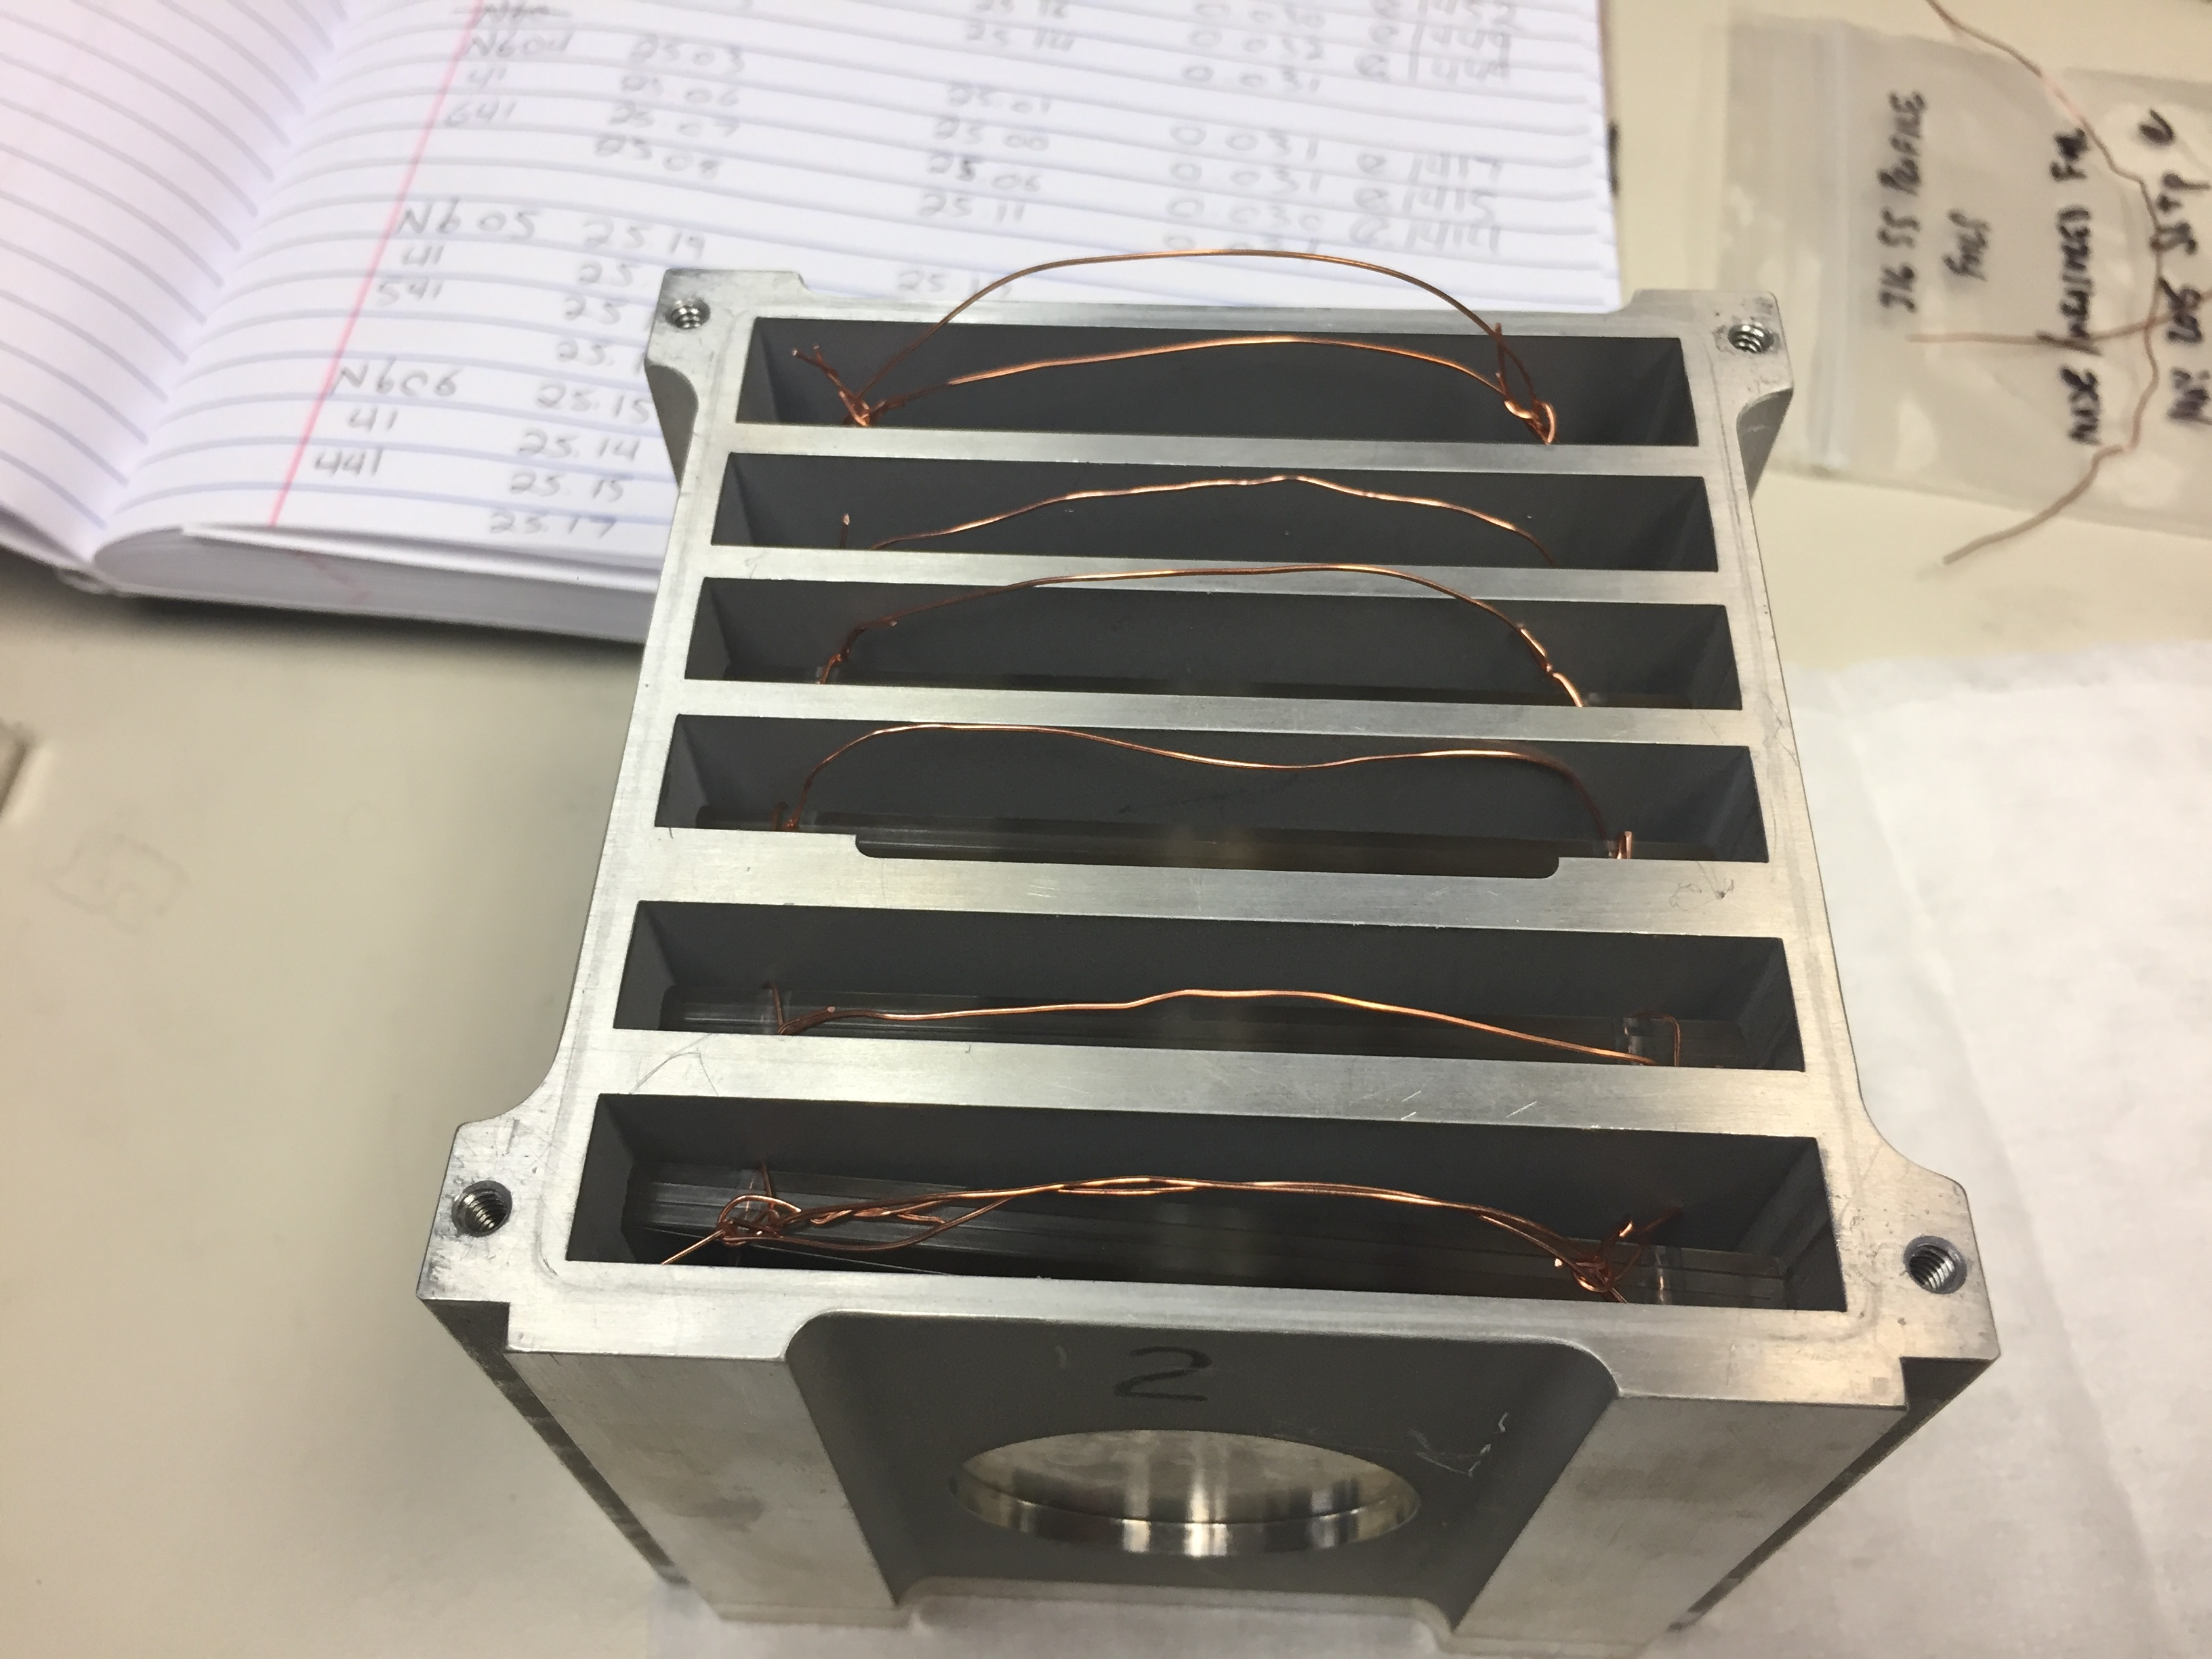
\includegraphics[scale=0.1,clip=true,trim=13cm 0cm 3cm 6cm]{./figures/IMG_1975.JPG}
 % IMG_1975.JPG: 3264x2448 pixel, 72dpi, 115.15x86.36 cm, bb=0 0 3264 2448
 \caption{Photograph of the assembled IPF target stack, before the stack's o-ring lid was sealed in place. The baling wire handles affixed to each bunch of Al+Cu+Nb foils are visible in each energy position, to facilitate removal of activated foils via robotic manipulators in the IPF hot cell. The circular Inconel beam entrance aperture is visible in the bottom center of the photograph.  }
 \label{fig:target_stack}
\end{figure}



% Please add the following required packages to your document preamble:
% \usepackage{booktabs}
\begin{table}
\centering
\caption{Specifications of the  target stack design in the present work. The proton beam enters the stack upstream of the 249.8 \micro m SS profile monitor, and is transported through the stack in the order presented here. The 6061 aluminum degraders have a measured density of approximately 2.80 g/cm$^3$, but their areal densities are not listed here due to the variance minimization techniques utilized  in this work.}
\label{tab:stack_table}
\begin{tabular}{@{}llll@{}}
\toprule
% Target Layer       & Nominal Thickness & Measured thickness (mg/cm\textasciicircum 2) & Thickness Uncertainty (\%) \\ \midrule
Target layer       & \begin{tabular}[c]{@{}l@{}}Measured \\ thickness\end{tabular} & \begin{tabular}[c]{@{}l@{}}Measured areal\\density (mg/cm$^2$)\end{tabular} & \begin{tabular}[c]{@{}l@{}}Areal density \\ uncertainty (\%)\end{tabular} \\ \midrule
SS profile monitor & 249.8 \micro m         & 194.555                                      & 0.290                      \\
Al-1               & 25.0 \micro m          & 6.519                                        & 0.724                      \\
Cu-1               & 61.3 \micro m          & 53.736                                       & 0.053                      \\
Nb-1               & 30.0 \micro m          & 23.205                                       & 0.073                      \\
Al Degrader 01     & 4.96 mm           & -                                            & -                          \\
Al-2               & 25.5 \micro m          & 6.484                                        & 0.364                      \\
Cu-2               & 61.8 \micro m          & 53.849                                       & 0.169                      \\
Nb-2               & 30.8 \micro m          & 22.905                                       & 0.166                      \\
Al Degrader 02     & 4.55 mm           & -                                            & -                          \\
Al-3               & 25.8 \micro m          & 6.472                                        & 0.314                      \\
Cu-3               & 61.5 \micro m          & 53.984                                       & 0.113                      \\
Nb-3               & 31.0 \micro m          & 22.906                                       & 0.235                      \\
Al Degrader 03     & 3.52 mm           & -                                            & -                          \\
Al-4               & 26.3 \micro m          & 6.505                                        & 0.407                      \\
Cu-4               & 61.3 \micro m          & 53.463                                       & 0.221                      \\
Nb-4               & 30.8 \micro m          & 22.550                                       & 0.245                      \\
Al Degrader 04     & 3.47 mm           & -                                            & -                          \\
Al-5               & 26.5 \micro m          & 6.479                                        & 0.296                      \\
Cu-5               & 61.5 \micro m          & 53.572                                       & 0.108                      \\
Nb-5               & 30.8 \micro m          & 22.110                                       & 0.248                      \\
Al Degrader 05     & 3.46 mm           & -                                            & -                          \\
Al-6               & 26.3 \micro m          & 6.475                                        & 0.624                      \\
Cu-6               & 62.0 \micro m          & 53.836                                       & 0.318                      \\
Nb-6               & 31.3 \micro m          & 22.120                                       & 0.130                      \\
SS profile monitor & 124.4 \micro m         & 101.336                                      & 0.226                      \\ \bottomrule
\end{tabular}
\end{table}





\subsection{Measurement of induced activities}\label{sec:spectroscopy}

\comment{get citation data for UNISAMPO}

Following activation, the Al, Cu, and Nb foils  were  transferred to the LANL TA-48 counting lab, where their induced activities could be measured via gamma ray spectroscopy.
For consistency, a single detector was used in this measurement, an ORTEC GEM Series  High-Purity Germanium (HPGe) detector.
The detector is a mechanically-cooled coaxial p-type HPGe with a 1 mm aluminum window, and a 49.2 mm diameter, 27.9 mm long crystal.
Samples were counted at fixed positions ranging 4.5 - 83.5  cm from the front face of the detector, with a series of standard calibration sources used to determine in-house energy, efficiency, and pileup calibrations for each position.
The foils were counted for a period of 2 weeks following EoB, to accurately quantify all induced activities.
An example gamma ray spectrum collected in such a fashion is shown in \autoref{fig:gspec}.
For all spectra collected, net peak areas were fitted using the gamma spectroscopy analysis code UNISAMPO \textred{(add UNISMPO citation)}, which has been shown to perform best in head-to-head comparisons with other common analysis codes \cite{Jackman2014}, due to its peak fitting algorithms and incorporation  of calibrated detector-specific peak shapes and widths. 

\begin{figure}
 \centering
 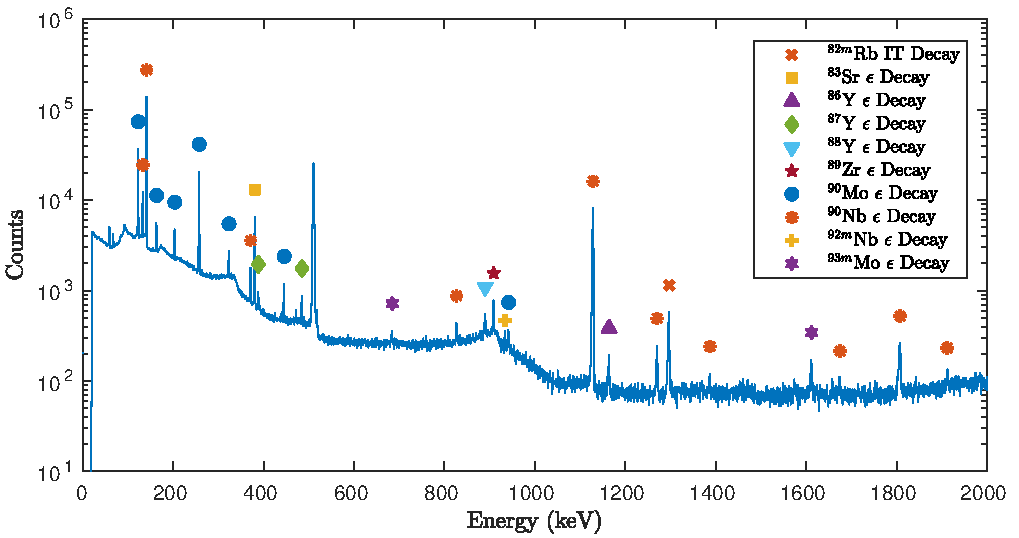
\includegraphics[width=6in]{./figures/sample_gspec.pdf}
 % sample_gspec.pdf: 489x257 pixel, 72dpi, 17.25x9.07 cm, bb=0 0 489 257
 \caption{Example gamma spectra, collected from an activated Nb foil at approximately 80 MeV, to monitor radioisotope production. While the majority of observed reaction products are visible in this spectrum, it is particularly noteworthy that the \ce{^{90}Mo} decay lines which form the basis of the \ce{^{93}Nb}(p,x)\ce{^{90}Mo} monitor reaction are high in intensity and clearly isolated from surrounding peaks, greatly aiding its activity quantification.}
 \label{fig:gspec}
\end{figure}


Following  acquisition, the decaying product nuclei corresponding to each observed peak in the collected spectra were identified.
The calibrated detector efficiencies, along with gamma ray intensities for each transition, were used to convert the net  counts in each fitted gamma ray photopeak into an activity for the activated isotopes and isomeric states.
For reference, the nuclear decay data used in this work is tabulated in \autoref{tab:nudat_table_monitors} and \autoref{tab:nudat_table_nb} of \ref{data}.
As nearly all of the product nuclei created in this work have multiple high-intensity gamma rays, each product nuclei had measurements of its present activity at multiple points in time (up to 2 weeks after EoB), as well as multiple independent activity measurements at each time point, based on each of its observed gamma rays.
The measured activity for each gamma ray possesses a total propagated uncertainty which is the quadrature sum of the uncertainty in  fitted peak areas, uncertainty in detector efficiency calibration, and uncertainty in the gamma ray branching ratio data.



\comment{Add 1st and 2nd order bateman stuff here, maybe cite Cetnar2006 also }



Since many of the reaction products populated by energetic protons are more than one decay off of stability, many of these are produced not only  directly by reactions, but also indirectly produced by decay down a mass chain.
To this end, it is useful to differentiate between the types of cross sections reported in this work. 
For the first observable product nuclei in a mass chain, its (p,x) cross section will be reported as a cumulative cross section ($\sigma_c$), which is the sum of direct production of that nucleus, as well as decay of its decay precursors and any other independent cross sections leading to that nucleus. 
In addition, cumulative cross sections will be reported whenever it is impossible to use decay spectroscopy to distinguish direct production of a nucleus from decay feeding.
For all remaining observed reaction products in the mass chain, independent cross sections ($\sigma_i$) will be reported, leaving solely direct nucleus production by subtracting out the feeding of decay precursors.



To convert these activities into cross sections, corrections must be made for the decay of the various reaction products in  between EoB and the spectrum acquisition, in order to calculate $A_0$, the initial activity at EoB.
The use of  multiple gamma rays at multiple points after EoB to calculate initial activities  for each observed product nucleus allows for a more accurate  determination of $A_0$ than simply basing its calculation off of a single gamma ray observation.
For the case of cumulative cross sections, EoB activities were quantified by fitting the activities observed at multiple time points $t$ (since EoB) to the well-known radioactive decay law.
% \begin{equation}
% A\pp{t} = A_0 e^{-\lambda t}
% \end{equation}
Nonlinear regression was used for this fitting process, minimizing on $\chi^2$ / degree of freedom, so that not only would the uncertainty-weighted EoB activities be fitted, but that a 1-$\sigma$ confidence interval in $A_0$ would be reported as as well.
As with the gamma ray intensities, all lifetimes used in this work are tabulated in \autoref{tab:nudat_table_monitors} and \autoref{tab:nudat_table_nb} of \ref{data}.
In the case of independent cross sections, a similar process was followed, quantifying $A_i\pp{0} = A_{i,0}$, the EoB activity of nuclide $i$, by instead regressing to the solutions to the Bateman equation:
\begin{equation}
A_n\pp{t} = \lambda_n \sum_{i=1}^n \left[  N_i\pp{0} \times \pp{\prod_{j=i}^{n-1}\lambda_j} \times \pp{\sum_{j=i}^n \dfrac{e^{-\lambda_j t}}{\prod_{i\neq j}^n \pp{\lambda_i - \lambda_j}}  }   \right]
\end{equation}
While higher-order terms were added if needed, typically for an isomeric state in a particular mass chain,  the second-order expansion ($n=2$) was often sufficient to quantify EoB activities in a mass chain, simplifying to:
\begin{equation}
A_2\pp{t} = \dfrac{A_{1,0}\lambda_2}{\lambda_1 - \lambda_2} \pp{e^{-\lambda_2 t} - e^{-\lambda_1 t}} + A_{2,0} e^{-\lambda_2 t}
\end{equation}
In these cases, the previously-quantified EoB activities from decay precursors ($A_{1,0}$, etc) would be substituted in, that the feeding contributions from decay could be separated and an independent cross section reported.
After quantifying the cumulative EoB activities at the top of a mass chain and all subsequent independent EoB activities, these will be later used to report the various cross sections for all observed reaction products and isomeric states. 











% \comment{Regex to replace table hard link with LaTeX cross-reference. - match w/ [T,t]able[^*}]   }


\subsection{Proton dosimetry}\label{sec:dosimetry}

% describe integral equation for converting activities to currents here

As discussed previously, accurate proton dosimetry is the most important factor in performing high-fidelity cross section measurements.
At the time of this work, the nondestructive beam current monitors in the LANSCE-IPF beamline possess resolution of 100 nAh.
For a low-current irradiation such as this work, where a nominal fluence of 200 nAh is desired, additional dosimetry is thus needed to accurately normalize quantified EoB activities into cross sections.
To this end, thin \ce{^{nat}Al} and \ce{^{nat}Cu} foils were included along with the \ce{^{nat}Nb} targets at each energy position, to provide another beam current monitor.
These foils have been recommended for use as proton monitor foils in the 30 \textless\ E$_\text{p}$ \textless\ 100 MeV regime by the IAEA, as the \ce{^{nat}Al}(p,x)\ce{^{22}Na}, \ce{^{nat}Al}(p,x)\ce{^{24}Na}, \ce{^{nat}Cu}(p,x)\ce{^{56}Co}, \ce{^{nat}Cu}(p,x)\ce{^{62}Zn}, and \ce{^{nat}Cu}(p,x)\ce{^{65}Zn} monitor reactions have been well-characterized for accurate proton fluence measurement \cite{gul2001charged}.
The recommended cross section values for each of these reactions were used in all calculations of proton fluence for the above monitor reactions.
Due to the large energy degradation between the front and  back of the target stack, a non-trivial broadening of the proton energy distribution is expected for all monitor and target foils.
As a result, the integral form of the well-known activation equation is used to accurately determine proton fluence ($I \Delta t $) in each monitor foil by convolving the IAEA recommended cross section values with the proton energy distribution:
% \begin{equation}
% A_0 = I\ \rho \Delta r \pp{1-e^{-\lambda \Delta t}} \int \sigma\pp{E} \dfrac{d\phi}{dE} dE
% \end{equation}
\begin{equation}
I \Delta t = \dfrac{A_0 \Delta t}{\rho \Delta r \pp{1-e^{-\lambda \Delta t}} \int \sigma\pp{E} \dfrac{d\phi}{dE} dE}
\end{equation}
where $A_0$ is the EoB activity for the monitor reaction product, $I$ is the proton current, $\rho \Delta r$ is the foil's areal density, $\lambda$ is the monitor reaction product's decay constant, $\Delta t$ is the length of irradiation, $\sigma\pp{E}$ is the IAEA recommended cross section at energy E, and $\frac{d\phi}{dE}$ is the differential proton fluence.
Using this formalism, the quantified EoB activities for each monitor reaction may be converted into a measured proton fluence at each energy position.


\comment{Add missing citations here}

The propagated uncertainty in proton fluence is calculated as the quadrature sum of the uncertainty in quantified EoB activity, uncertainty in the duration of irradiation (conservatively estimated at 60 s, to account for any transient changes in beam current), uncertainty in foil areal density, uncertainty in monitor product half-life (included, but normally negligible), uncertainty in IAEA recommended cross section, and uncertainty in proton fluence.
Of these, the first four contributions are all easily quantified in the preparation and execution of a stacked target irradiation;  the last two contributions prove to be more nuanced, however.
The uncertainty in proton fluence for irradiated monitor foils is derived from statistical uncertainty in the modeling of proton transport in the stack irradiation, discussed in \autoref{sec:proton_transport}.
The uncertainty in IAEA recommended cross section values must be estimated indirectly, as no uncertainty in the  recommended cross sections is provided in the current IAEA evaluation.
Fortunately, the recommended cross section values for each monitor reaction tend to match one of the   selected experimental data sets used in their evaluation almost perfectly.
Since these data sets have listed uncertainties in the original manuscripts, uncertainties in  IAEA recommended cross section values have been estimated by the uncertainty in the data set most closely matching the  IAEA recommended  values.
For the monitor reactions employed in this work, these data sets are G. Steyn (1990) for  \ce{^{nat}Al}(p,x)\ce{^{22}Na} \textred{(insert Steyn citation here)}, M. Uddin (2004) for \ce{^{nat}Al}(p,x)\ce{^{24}Na} \cite{Uddin2004}, and S. Mills (1992) for \ce{^{nat}Cu}(p,x)\ce{^{56}Co}, \ce{^{nat}Cu}(p,x)\ce{^{62}Zn}, and \ce{^{nat}Cu}(p,x)\ce{^{65}Zn} \cite{Mills1992}.




\subsection{Proton transport calculations}\label{sec:proton_transport}


Initial estimates of the proton beam energy in all foils were calculated using the Anderson \& Ziegler (A\&Z) stopping power formalism \cite{Andersen_Ziegler_1977,Ziegler1985,Ziegler1999}.
These estimates of average beam energy in each foil are useful for the preliminary stack design, as the A\&Z calculation provide reasonable approximations of 1-D proton transport due to its treatment of ionization and multiple Coulomb scattering. 
However, for final energy determination and analysis, a more rigorous method of proton transport is needed.
The Monte Carlo N-Particle transport code MCNP6.1 was used for simulation of the full 3-D target stack, and is used to calculate a full proton energy distribution for each stack position   \cite{Goorley2012}.
In addition, MCNP6 provides a far more robust method of proton transport, as it is able to account for beam losses due to reactions, as well as production of secondary particles.
As it is a Monte Carlo-based code, the uncertainty in energy distribution scales inversely with the number of source protons simulated - $10^8$ source protons were used for all simulations, which places the statistical uncertainty in proton energy distributions at less than 0.01\%.


The ability to model the full energy distribution in each target position is vital for stacked target irradiations, due to the progressively larger energy straggling towards the rear of the stack.
The initial proton beam has a finite energy spread (an approximately 0.1 MeV Gaussian width at 100 MeV), and since stopping power for charged particles is inversely proportional to their energy, the low-energy tail of the energy distribution is degraded more in each stack element than the high-energy tail.
This effect compounds as one moves towards the rear of the stack, with the effect of a significantly broadened low-energy tail relative to the high-energy tail, and a progressively larger net shift of the centroid to a lower energy than the peak of the energy distribution. 
% For each foil in the target stack, 
To account for this increasing energy uncertainty, a suitably representative energy must be established for  each foil in the target stack.
In this work, the flux-weighted average proton  energy in each foil, $\langle E \rangle$,  represents the energy centroid for protons in a target stack component, calculated using the energy distributions $\frac{d\phi}{dE}$ from MCNP6 modeling of proton transport:
\begin{equation}
\langle E \rangle = \dfrac{{\displaystyle\int E \dfrac{d\phi}{dE} dE}}{{\displaystyle\int \dfrac{d\phi}{dE} dE}}
\end{equation}
Likewise, to represent the energy uncertainty for each stack position, the full width at half maximum (FWHM) of the MCNP6-modeled energy distribution is chosen for each energy position reported.
While most experimental uncertainties are reported at the 1$\sigma$ level, the $\approx2.3\sigma$ FWHM is used here to ensure at the 98\% confidence interval that this width includes  the \enquote{true} energy center-of-mass.





Based on the recent work of Graves \etal, the \enquote{variance minimization} techniques they outline have been employed here, to further reduce the uncertainty in proton energy assignments     \cite{Graves2016}.
This method is based on the assumption that the independent measurements of proton fluence from the 5 monitor reactions used in this work should all be consistent at each energy position.
If the monitor reaction cross sections and MCNP6 - modeled energy distributions are both accurate, then any disagreement in the  observed proton fluences is due to a systematic uncertainty in the stack design, namely, the areal densities of the stack components \cite{Graves2016,Marus2015}. 
This disagreement is minor at the front of the stack, and gets progressively worse as the beam is degraded, due to the compounded effect of systematic uncertainties in stack areal densities.



To correct for this, variance minimization techniques were employed here to correct for uncertainties in  the characterization of the stack components, the largest cause of uncertainties in energy and  fluence assignments.
Due to the difficulty of characterizing uncertainty in areal density in the Kapton tape, the areal density of these layers were varied uniformly in MCNP6 simulations by up to $\pm$25\% of nominal values, but this had negligible impact on improving monitor reaction disagreement.
This is due to the minor impact that their areal density has on beam degradation, relative to the thick 6061 aluminum degraders (nominal 3-5 mg/cm$^2$, relative to nominal 1000-1400 mg/cm$^2$).
As such,  the areal density of each of the 6061 aluminum degraders  were varied uniformly in MCNP6 simulations  by a factor of up to $\pm$25\% of nominal values, to find the effective density which minimized variance in the measured proton fluence at the lowest energy position (Al-6, Cu-6).
This lowest energy position was chosen as a minimization candidate, as it is most sensitive to systematic uncertainties in stack design.
The results of this minimization technique, shown in \autoref{fig:variation_curve}, indicate a clear minimum in proton fluence variance for flux-weighted average 41.34 MeV protons entering the last energy position, approximately 2 MeV lower than the nominal MCNP6 simulations, and approximately 3 MeV lower than nominal A\&Z calculations, both of which used the nominal 2.80 g/cm$^3$ measured density of the 6061 aluminum degraders.
This energy corresponds to a 6061 aluminum areal density of 2.53\% greater than nominal measurements, and serves as a lump correction for other minor systematic uncertainties in stack design, including stack areal densities and incident beam energy.



The impact of this variance minimization may  clearly be seen in   \autoref{fig:variance_mins}.
As expected, the 2.53\% increase in 6061 aluminum areal density has an almost negligible impact on the higher-energy positions, but causes a progressively larger downshift  in proton energies at the later energy positions.
In addition, as one moves to the rear energy positions, the disagreement in the independent proton fluence measurements is reduced.
It is worth noting that the proton fluence measured by the \ce{^{nat}Al}(p,x)\ce{^{22}Na} monitor reaction is consistently higher in magnitude than all other monitor channels, with an increasing disparity at higher energies.
This phenomenon is observed for the \ce{^{nat}Cu}(p,x)\ce{^{56}Co} monitor reaction as well, though to a much smaller degree.
In both cases, this disparity is caused by the fact that both of these monitor reactions may also form the \ce{^{22}Na} and \ce{^{56}Co} reaction products through contamination by secondary neutron (n,x) channels, increasing the apparent fluence as observed by these monitor reactions.
Since no method for reliably separating the fraction of \ce{^{22}Na} and \ce{^{56}Co} activities induced through (n,x) exists, the fluences predicted by these monitor channels are not used in the final determination of the proton fluence seen by Nb foils. 
The fact that this \enquote{extra fluence} diminishes at lower energy is likely attributed to the fact that the \ce{^{nat}Al}(p,x)\ce{^{22}Na} and \ce{^{nat}Cu}(p,x)\ce{^{56}Co} have energetic thresholds of 23.35 and 36.76 MeV, respectively - the fraction of secondary neutrons produced by (p,xn)  which are energetic enough to populate the  \ce{^{22}Na} and \ce{^{56}Co} reaction products at the lower energy positions becomes progressively smaller.
This serves as an example of the importance of selecting monitor reaction products inaccessible through (n,x) channels, as noted previously.
However,  the fact that both monitor reactions measure consistently higher fluence than the other channels on each foil builds confidence that the monitor reactions accurately indicate the presence of the secondary neutron flux.







\begin{figure}
 \centering
 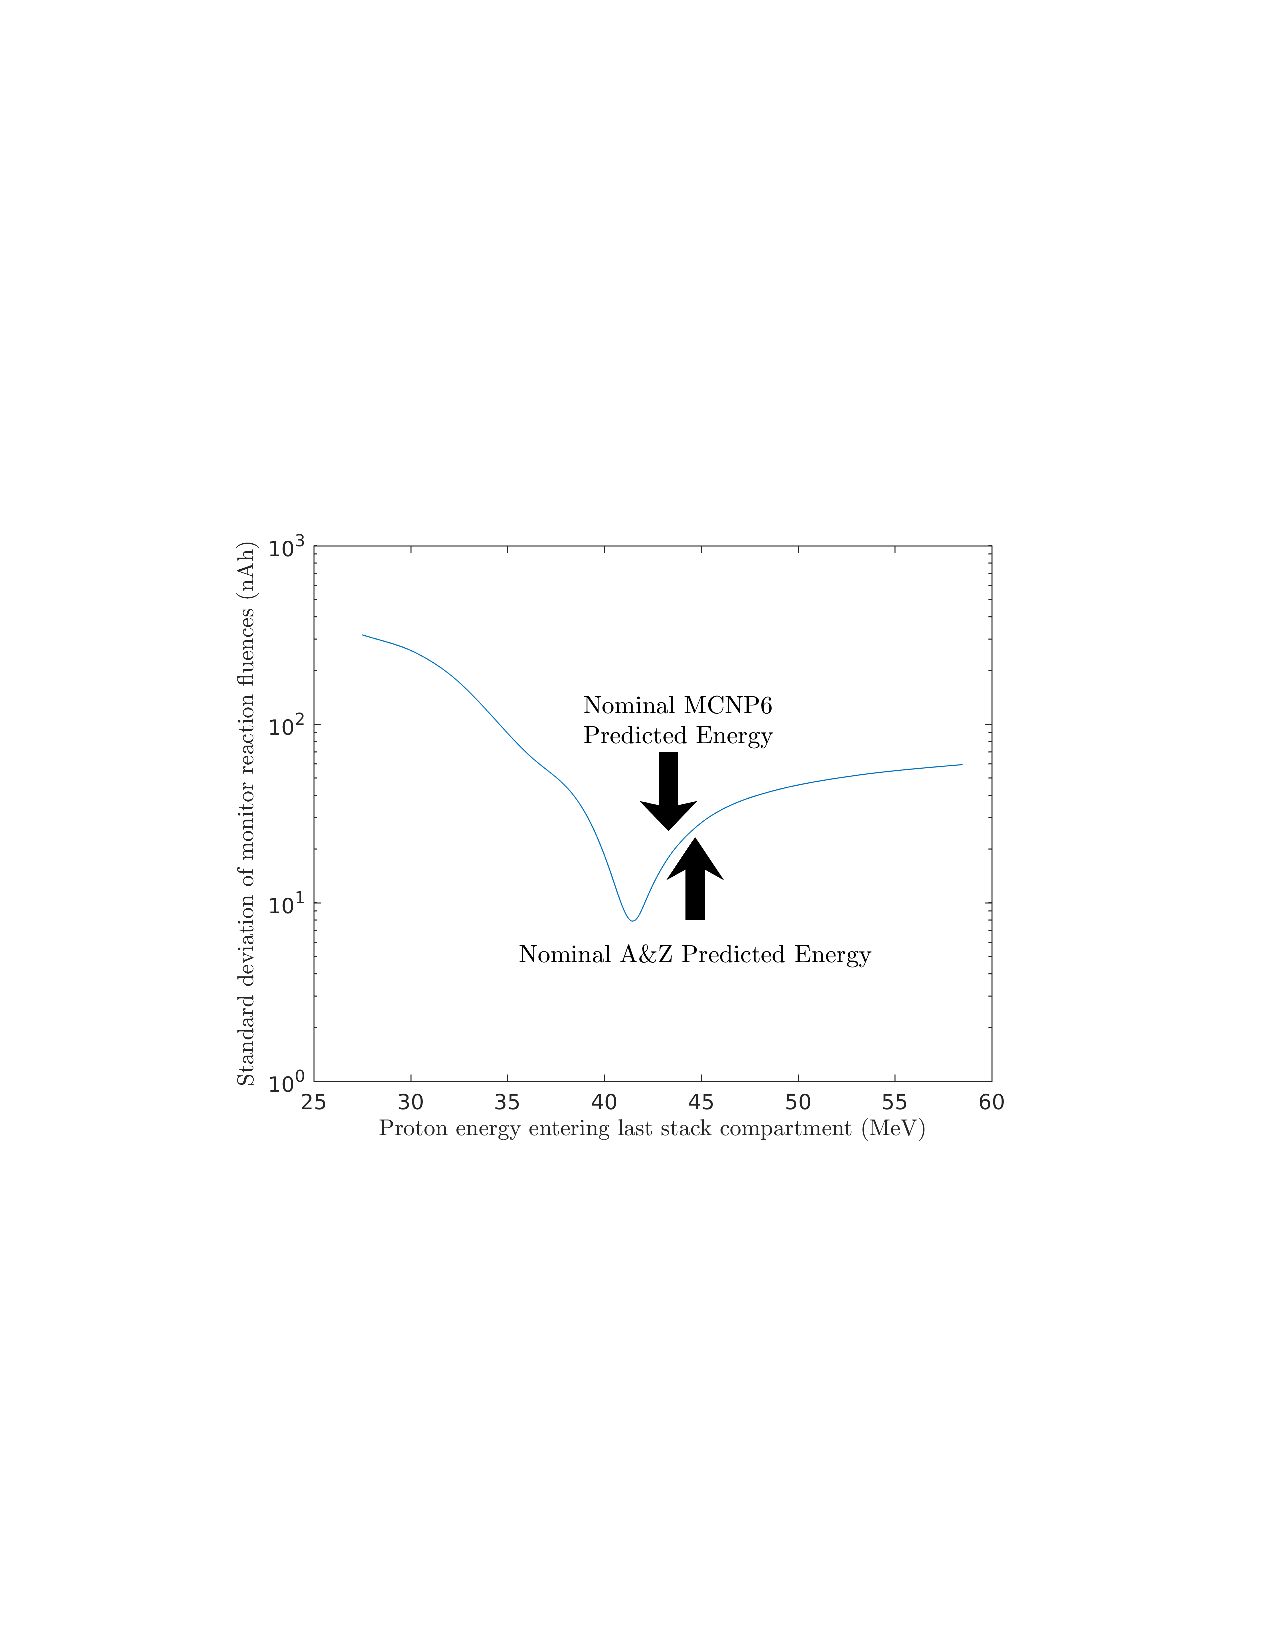
\includegraphics[clip=true,trim=1.5in 3.4in 1.8in 3.5in, scale=0.8]{./figures/variation_curve.pdf}
 % variation_curve.pdf: 612x792 pixel, 72dpi, 21.59x27.94 cm, bb=0 0 612 792
 \caption{Result of variance minimization, performed by varying the degrader density in MCNP6 simulations of the target stack.  A flux-weighted average proton energy of 41.34 MeV entering the last energy position creates a clear minimum in observed reaction fluence variance, corresponding to an areal density 2.53\% greater than nominal. The variance minimum occurring at a lower incident energy than nominal MCNP6 and A\&Z calculations indicates that there exists an additional systematic beam degradation not accounted for in modeling of proton transport in the stack design.}
 \label{fig:variation_curve}
\end{figure}


\begin{figure*}
    \centering
    \begin{subfigure}[t]{0.49\textwidth}
        \centering
%         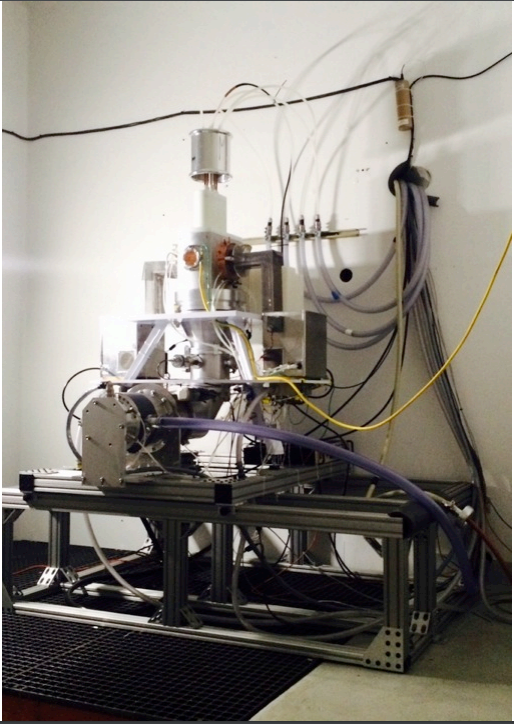
\includegraphics[width=\columnwidth]{./figures/Capture.PNG}
        \subfigimg[scale=0.59]{a)}{./figures/before_minimization_plot.pdf}
%         \caption{ Decay curve for the isomeric transition of \ce{^{115m}In}.}
         \refstepcounter{subfigure}\label{fig:before_minimization}
    \end{subfigure}%
     \begin{subfigure}[t]{0.49\textwidth}
        \centering
%         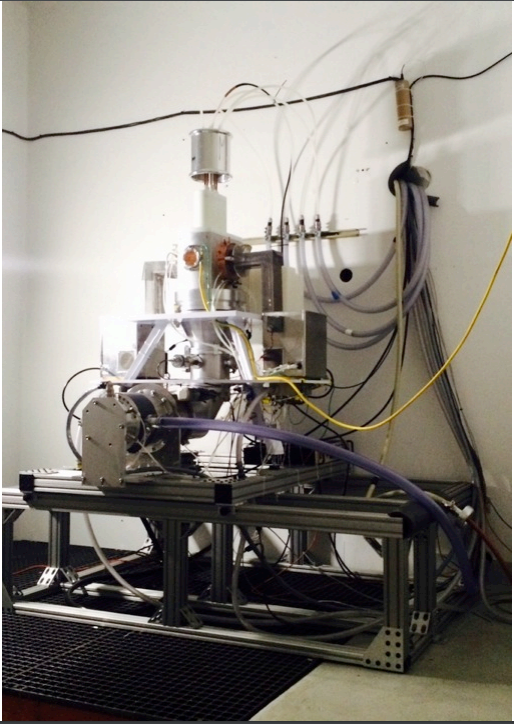
\includegraphics[width=\columnwidth]{./figures/Capture.PNG}
%         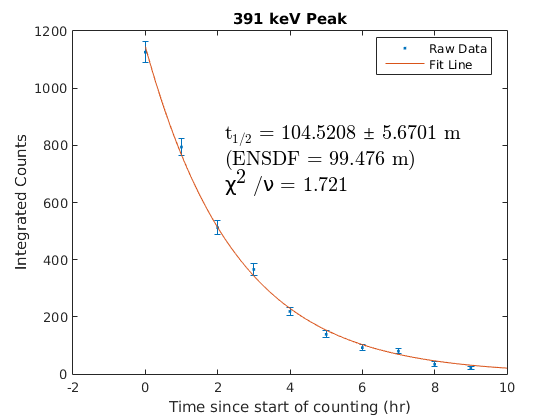
\includegraphics[scale=0.6]{./figures/391keV_curve2.png}
        \subfigimg[scale=0.59]{b)}{./figures/after_minimization_plot.pdf}
%         \caption{ Decay curve for the isomeric transition of \ce{^{113m}In}.}
         \refstepcounter{subfigure}\label{fig:after_minimization}
    \end{subfigure}%
    \caption{Results of variance minimization through enhancement of 6061 aluminum effective areal density by 2.53\%. A noticeable reduction of variance in measured proton fluence is seen, in particular at the low-energy rear positions of the stack. The \enquote{extra fluence} observed in the  \ce{^{nat}Al}(p,x)\ce{^{22}Na} and \ce{^{nat}Cu}(p,x)\ce{^{56}Co} monitor channels is caused by activation through (n,x) reactions from the secondary neutron flux. By excluding these contaminated channels, the remaining 3 independent monitor reactions serve to minimize uncertainty in stack energy assignments and incident fluence.}
     \label{fig:variance_mins}
\end{figure*}

Using this variance minimized degrader density, the final incident proton energy energy distributions $\frac{d\phi}{dE}$ from MCNP6 simulation are shown for the 6 irradiated Nb foils in \autoref{fig:Nb_ptallies}. 
As expected, the energy distribution becomes increasingly more broadened at the lower energy positions, as result of the beam energy degradation.
In addition, as the beam becomes more degraded, the magnitude of the peak of each energy distribution (as well as the integral of each distribution) is reduced in magnitude, as beam fluence is lost due to scattering, and the peak-to-low-energy-tail-ratio increases as more  secondary protons are produced upstream.
As with the monitor foils, these distributions were used to calculate the  energy centroid  (as the  flux-weighted average proton  energy) and  uncertainty (as the FWHM of the distribution) for the final proton energy assignment of each Nb foil.





An enhanced version of the final monitor reaction fluences may be seen in \autoref{fig:fluence_plot}, which shows the  \ce{^{nat}Al}(p,x)\ce{^{24}Na} observed fluence (the upper set of points), and the uncertainty-weighted average fluence from the  \ce{^{nat}Cu}(p,x)\ce{^{62}Zn} and \ce{^{nat}Cu}(p,x)\ce{^{65}Zn} monitor reactions (the lower set of points).
To determine the final fluence assignments for the Nb foils, uncertainty-weighted linear regression was used to fit the various fluence measurements, minimizing on $\chi^2$ / degree of freedom, so that  a 95\% confidence interval in fluence would be reported as as well.
As with the FWHM, a greater than 1$\sigma$ confidence interval is used for reporting fluence uncertainty to avoid an unrealistically small fluence confidence interval, based on the spread in observed fluence from Al and Cu monitor foils.
% The fluence and 2$\sigma$ uncertainties from this weighted-fit line are thus used in calculations of the various Nb(p,x) cross sections



\begin{figure}
 \centering
 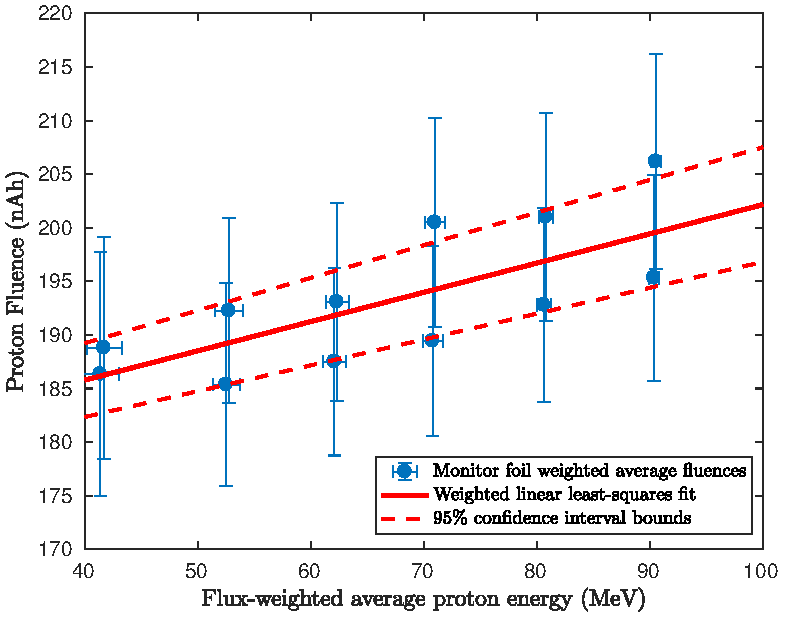
\includegraphics[scale=.8]{./figures/fluence_plot.pdf}
 % Nb_ptallies.pdf: 380x298 pixel, 72dpi, 13.41x10.51 cm, bb=0 0 380 298
 \caption{Final weighted-fit proton fluences throughout the target stack, based on the variance-minimized observed fluence from the the  \ce{^{nat}Al}(p,x)\ce{^{24}Na}, \ce{^{nat}Cu}(p,x)\ce{^{62}Zn}, and \ce{^{nat}Cu}(p,x)\ce{^{65}Zn} monitor reactions. A 95\% ($2\sigma$) confidence interval is reported in the fitted proton fluence, to ensure a realistic uncertainty in fluence, which encompasses the true absolute fluence. A clear loss of fluence  is visible, dropping by approximately 8.1\% from the incident fluence of 202.2 nAh over the length of the target stack.  This is due to a combination of beam utilization, as well as scattering.}
 \label{fig:fluence_plot}
\end{figure}





\begin{figure}
 \centering
 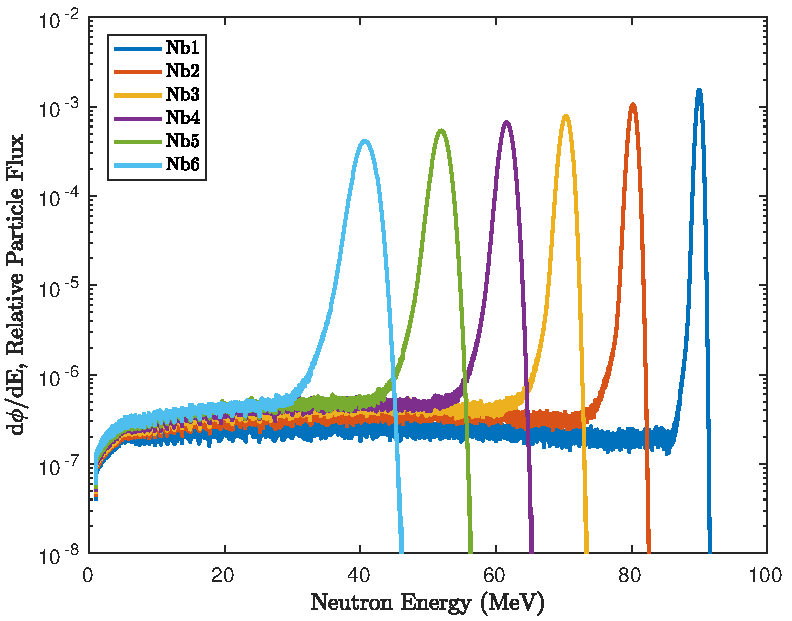
\includegraphics[scale=.8]{./figures/Nb_ptallies.pdf}
 % Nb_ptallies.pdf: 380x298 pixel, 72dpi, 13.41x10.51 cm, bb=0 0 380 298
 \caption{Final variance minimized incident proton energy distributions for the Nb foils, as simulated in MCNP6. The distribution tallies in each foil are all normalized to be per source proton, which was $10^8$ in all simulations. As the beam is degraded, proton energy distributions become visibly broadened due to straggling, and drop in magnitude due to scattering losses.}
 \label{fig:Nb_ptallies}
\end{figure}


% \begin{equation}
% R = N_T \int_0^{E_{max}} \sigma(E) \dfrac{d\phi}{dE} dE
% \end{equation}





\subsection{Calculation of measured cross sections}\label{sec:calcs_sec}

%  include 1st and 2nd order bateman stuff here

XXXXXX

\comment{Double check this equation from my scratch work at LBL} 

% \begin{align}
% N_{\gamma} &= N_D \epsilon_\gamma I_\gamma \\
% &=  \epsilon_\gamma I_\gamma  \dfrac{N_T \sigma\pp{\bar{E}} \phi\pp{\bar{E}} }{\lambda}\pp{1 - e^{-\lambda t_i}}  e^{-\lambda t_d} \pp{1 - e^{-\lambda t_c}} \nonumber
% \end{align}



% \autoref{eqn:single_xs_eqn} can be used to determine the unknown (n,p) cross sections relative to the well-known \ce{^{115}In}(n,n')\ce{^{115m}In} and \ce{^{113}In}(n,n')\ce{^{113m}In} inelastic scattering cross sections since the Zn and Ti samples were co-irradiated with indium foils.
% This approach has a number of advantages since the result is independent of neutron flux and only depends on the relative detector efficiencies at each gamma-ray energy.
 

\subsection{Systematic uncertainties}

XXXXXX




\section{Results}


XXXXXX

          
% \section{Discussion}

\comment{Feel free to suggest / add other language describing medical radionuclide applications, or radiochemical separations here.}


% XXXXXX
 
 
 
 \section{Conclusions}

XXXXXX


 
 \section{Acknowledgements}
 
%  Stephen Graves - consulting for methodology, guidance.
 
 Michael Gallegos and Don Dry in the C-NR Countroom, David Reass and Mike Connors at IPF, and the LANSCE Accelerator Operations staff 
 
 This research used the Savio computational cluster resource provided by the Berkeley Research Computing program at the University of California, Berkeley (supported by the UC Berkeley Chancellor, Vice Chancellor for Research, and Chief Information Officer).
 
 
 \comment{Please provide me here with all relevant contract / grant / fellowship / funding ID numbers.}
 
%  We would like to particularly point out the crucial role played by Cory Waltz in the design and commissioning of the HFNG.
%  We wish to thank Marc Garland and Saed Mirzadeh for discussions regarding the use of neutron generators for isotope production.
%  We acknowledge Glenn Jones of G\&J Jones Enterprises of Dublin, CA for the construction  of the High Flux Neutron Generator. 
%  Lastly, we would like to acknowledge the students in the Nuclear Reactions and Radiation (NE102) laboratory course at UC Berkeley who participated in these experiments, including Joe Corvino, Nizelle Fajardo, Scott Parker and Evan Still.  
%  
%  This work has been carried out at the University of California, Berkeley, and performed under the auspices of the U.S. Department of Energy by Lawrence Livermore National Laboratory under contract \# DE-AC52-07NA27344 and Lawrence Berkeley National Laboratory under contract \# DE-AC02-05CH11231.
% Funding has been provided from the US Nuclear Regulatory Commission, the US Nuclear Data Program, the Berkeley Geochronology Center, NSF ARRA Grant \# EAR-0960138, the University of California Laboratory Fees Research Grant \# 12-LR-238745, and  DFG Research Fellowship \# RU 2065/1-1.



% \pagebreak
% 
% \onecolumn
% 
\appendix


\section{Decay data} \label{data}
% 
% % \begin{longtable}{|c|c|c|c|c|} 
% % \caption{My caption}
% % \label{tab:dummy}
% % % \begin{tabular}{|c|c|c|c|c|}
% %    \hline
% %  
% % \end{longtable}
Table of decay data  for observed gamma rays. 
The  values for lifetime and gamma ray branching ratios  listed here were used in all calculations of measured cross sections \cite{Wang2017,Dong2015,Dong2014,JUNDE2008787,Junde2011,Bhat1998,Nesaraja2010,BAGLIN2002,Browne2013,Zuber20151,NICHOLS2012973,Singh2007,Browne2010,Tuli2003,McCutchan2015,Singh2014,NEGRET20151,Johnson2015,McCutchan2014,Singh2013,Browne1997,Baglin2013,Baglin2012}. 

\comment{add citation for NDS A=22,24,93}

\comment{I had to remove about 30 of the lines I used from this table (removing the weakest lines in nuclides with even more lines than shown here, but never removing lines in nuclides with only 2 or less), as even splitting the data into 2 tables created tables too large to fit on a single page.  My purpose here was 1) to show that I used multiple lines to quantify each nuclide (increasing confidence in results), and 2) to list all the used \ce{^{90}Mo} lines, since they form the basis of it as a monitor.  Is this good as is, or should it be pared down even more?}


% Preview source code for paragraph 0

\begin{table}[ht]
\centering
\caption{Decay data for gamma rays observed in \ce{^{nat}Al}(p,x) and \ce{^{nat}Cu}(p,x).}
\label{tab:nudat_table_monitors}
\begin{tabular}{@{}llll@{}}
\toprule
% \begin{tabular}{|c|c|c|c|}
% \hline 
Nuclide & Half-life & E$_\gamma$ (keV) & I$_\gamma$ (\%)\\
\midrule
\ce{^{22}Na} & 2.6018(22) y & 1274.537 & 99.940(14)\\
 
\ce{^{24}Na} & 14.997(12) h & 1368.626 & 99.9936(15)\\
 
\ce{^{51}Cr} & 27.704(3) d & 320.0824 & 9.910(10)\\
 
\ce{^{52m}Mn} & 21.1(2) m & 1434.0600 & 98.2(5)\\
 
\ce{^{52}Mn} & 5.591(3) d & 744.233 & 90.0(12)\\
 
 & 5.591(3) d & 935.544 & 94.5(13)\\
 
 & 5.591(3) d & 1246.278 & 4.21(7)\\
 
 & 5.591(3) d & 1434.092 & 100.0(14)\\
 
\ce{^{54}Mn} & 312.20(20) & 834.848 & 99.9760(10)\\
 
\ce{^{55}Co} & 17.53(3) h & 477.2 & 20.2(17)\\
 
 & 17.53(3) h & 931.1 & 75.0(35)\\
 
 & 17.53(3) h & 1316.6 & 7.1(3)\\
 
 & 17.53(3) h & 1408.5 & 16.9(8)\\
 
\ce{^{56}Ni} & 6.075(10) d & 158.38 & 98.8(10)\\
 
 & 6.075(10) d & 269.50 & 36.5(8)\\
 
 & 6.075(10) d & 480.44 & 36.5(8)\\
 
 & 6.075(10) d & 749.95 & 49.5(12)\\
 
 & 6.075(10) d & 811.85 & 86.0(9)\\
 
 & 6.075(10) d & 1561.80 & 14.0(6)\\
 
\ce{^{56}Co} & 77.236(26) d & 846.770 & 99.9399(2)\\
 
%  & 77.236(26) d & 977.372 & 1.421(6)\\
 
 & 77.236(26) d & 1037.843 & 14.05(4)\\
 
 & 77.236(26) d & 1238.288 & 66.46(12)\\
 
 & 77.236(26) d & 1360.212 & 4.283(12)\\
 
 & 77.236(26) d & 1771.357 & 15.41(6)\\
 
\ce{^{57}Ni} & 35.60(6) h & 127.164 & 16.7(5)\\
 
 & 35.60(6) h & 1377.63 & 81.7(24)\\
 
 & 35.60(6) h & 1757.55 & 5.75(20)\\
 
 & 35.60(6) h & 1919.52 & 12.3(4)\\
 
\ce{^{57}Co} & 271.74(6) d & 122.06065 & 85.60(17)\\
 
 & 271.74(6) d & 136.47356 & 10.68(8)\\
 
\ce{^{58}Co} & 70.86(6) d & 810.7593 & 99.450(10)\\
 
 & 70.86(6) d & 863.951 & 0.686(10)\\
 
%  & 70.86(6) d & 1674.725 & 0.517(10)\\
 
\ce{^{59}Fe} & 44.495(9) d & 1099.245 & 56.5(18)\\
 
 & 44.495(9) d & 1291.590 & 43.2(14)\\
 
\ce{^{60}Co} & 5.2714(5) y & 1173.228 & 99.85(3)\\
 
 & 5.2714(5) y & 1332.492 & 99.9826(6)\\
 
\ce{^{61}Cu} & 3.339(8) h & 282.956 & 12.2(2.2)\\
 
 & 3.339(8) h & 373.050 & 2.1(4)\\
 
%  & 3.339(8) h & 588.605 & 1.17(21)\\
 
 & 3.339(8) h & 656.008 & 10.8(20)\\
 
 & 3.339(8) h & 1185.234 & 3.7(7)\\
 
\ce{^{62}Zn} & 9.193(15) h & 243.36 & 2.52(23)\\
 
 & 9.193(15) h & 246.95 & 1.90(18)\\
 
 & 9.193(15) h & 260.43 & 1.35(13)\\
 
%  & 9.193(15) h & 304.88 & 0.29(3)\\
 
%  & 9.193(15) h & 349.60 & 0.45(4)\\
 
 & 9.193(15) h & 394.03 & 2.24(17)\\
 
 & 9.193(15) h & 548.35 & 15.3(14)\\
 
 & 9.193(15) h & 596.56 & 26.0(20)\\
 
%  & 9.193(15) h & 637.41 & 0.25(3)\\
 
\ce{^{64}Cu} & 12.701(2) h & 1345.77 & 0.475(11)\\
 
\ce{^{65}Zn} & 243.93(9) d & 1115.539 & 50.04(10)\\
\bottomrule
\end{tabular}
\end{table}



\begin{table}[ht]
\centering
\caption{Decay data for gamma rays observed in \ce{^{nat}Nb}(p,x).}
\label{tab:nudat_table_nb}
\begin{tabular}{@{}llll@{}}
\toprule
% \begin{tabular}{|c|c|c|c|}
% \hline 
Nuclide & Half-life & E$_\gamma$ (keV) & I$_\gamma$ (\%)\\
\midrule
\ce{^{82m}Rb} & 6.472(6) h & 554.35 & 62.4(9)\\
 
 & 6.472(6) h & 619.11 & 37.98(9)\\
 
%  & 6.472(6) h & 698.37 & 26.3(7)\\
 
 & 6.472(6) h & 776.52 & 84.39(21)\\
 
 & 6.472(6) h & 1044.08 & 32.07(8)\\
 
%  & 6.472(6) h & 1317.43 & 23.7(6)\\
 
\ce{^{83}Sr} & 32.41(3) h & 418.37 & 4.2(3)\\
 
 & 32.41(3) h & 762.65 & 26.7(22)\\
 
\ce{^{85m}Y} & 4.86(13) h & 231.7 & 22.8(22)\\
 
\ce{^{85}Y} & 2.68(5) h & 231.65 & 84(9)\\
 
 & 2.68(5) h & 913.89 & 9.0(9)\\
 
\ce{^{86}Zr} & 16.5(1) h & 242.8 & 95.84(2)\\
 
 & 16.5(1) h & 612.0 & 5.8(3)\\
 
% \ce{^{86}Y} & 14.74(2) h & 187.87 & 1.26(4)\\
\ce{^{86}Y}  & 14.74(2) h & 443.13 & 16.9(5)\\

 
%  & 14.74(2) h & 190.80 & 1.01(3)\\
 
%  & 14.74(2) h & 307.00 & 3.47(8)\\
 
%  & 14.74(2) h & 443.13 & 16.9(5)\\
 
%  & 14.74(2) h & 580.57 & 4.78(14)\\
 
%  & 14.74(2) h & 608.29 & 2.01(15)\\
 
 & 14.74(2) h & 627.72 & 32.6(1)\\
 
%  & 14.74(2) h & 703.33 & 15.4(4)\\
 
%  & 14.74(2) h & 709.90 & 2.62(8)\\
 
%  & 14.74(2) h & 767.63 & 2.4(3)\\
 
%  & 14.74(2) h & 835.67 & 4.4(6)\\
 
%  & 14.74(2) h & 1024.04 & 3.79(17)\\
 
 & 14.74(2) h & 1076.63 & 82.5(4)\\
 
 & 14.74(2) h & 1153.05 & 30.5(9)\\
 
%  & 14.74(2) h & 1163.03 & 1.18(4)\\
%  
%  & 14.74(2) h & 1253.11 & 1.53(5)\\
 
%  & 14.74(2) h & 1349.15 & 2.95(9)\\
 
 & 14.74(2) h & 1854.38 & 17.2(5)\\
 
 & 14.74(2) h & 1920.72 & 20.8(7)\\
 
\ce{^{87}Zr} & 1.68(1) h & 380.79 & 62.79(10)\\
 
 & 1.68(1) h & 1227.0 & 2.80(4)\\
 
\ce{^{87m}Y} & 13.37(1) h & 380.79 & 78.05(8)\\
 
\ce{^{87}Y} & 79.8(3) h & 388.5276 & 82.2(7)\\
 
 & 79.8(3) h & 484.805 & 89.8(9)\\
 
\ce{^{88}Zr} & 83.4(3) d & 392.87 & 97.29(14)\\
 
\ce{^{88}Y} & 106.627(21) d & 898.042 & 93.7(3)\\
 
 & 106.627(21) d & 1836.063 & 99.2(3)\\
 
\ce{^{89m}Nb} & 66(2) m & 588.0 & 95.57(13)\\
 
\ce{^{89}Nb} & 2.03(7) h & 1511.4 & 1.9(4)\\
 
 & 2.03(7) h & 1627.2 & 3.5(7)\\
 
 & 2.03(7) h & 1833.4 & 3.3(7)\\
 
\ce{^{89}Zr} & 78.41(12) h & 909.15 & 99.04(3)\\
 
 & 78.41(12) h & 1713.0 & 0.745(13)\\
 
%  & 78.41(12) h & 1744.5 & 0.123(4)\\
 
\ce{^{90}Mo} & 5.56(9) h & 122.370 & 64(3)\\
 
 & 5.56(9) h & 162.93 & 6.0(6)\\
 
 & 5.56(9) h & 203.13 & 6.4(6)\\
 
 & 5.56(9) h & 257.34 & 78(4)\\
 
 & 5.56(9) h & 323.20 & 6.3(6)\\
 
 & 5.56(9) h & 472.2 & 1.42(16)\\
 
 & 5.56(9) h & 941.5 & 5.5(7)\\
 
\ce{^{90}Nb} & 14.6(5) h & 132.716 & 4.13(4)\\
 
 & 14.6(5) h & 141.178 & 66.8(7)\\
 
%  & 14.6(5) h & 890.64 & 1.80(4)\\
 
 & 14.6(5) h & 1611.76 & 2.38(7)\\
 
%  & 14.6(5) h & 1913.194 & 1.280(17)\\
 
\ce{^{91m}Nb} & 60.86(22) d & 104.62 & 0.574(1)\\
 
 & 60.86(22) d & 1204.67 & 2.0(3)\\
 
\ce{^{92m}Nb} & 10.15(2) d & 912.6 & 1.78(10)\\
 
 & 10.15(2) d & 934.44 & 99.15(4)\\
 
\ce{^{93m}Mo} & 6.85(7) d & 263.049 & 57.4(11)\\
 
 & 6.85(7) d & 684.693 & 99.9(8)\\
 
 & 6.85(7) d & 1477.138 & 99.1(11)\\
\bottomrule
\end{tabular}
\end{table}


% 
% 
\section{Measured excitation functions} \label{fit_figures}

Figures of the cross sections measured in this work are presented here, in comparison with literature data \cite{Albouy1963,PhysRev.162.1055,PhysRevC.6.1235,Grutter1982,Greenwood1984,Aleksandrov1987,levkovski1991cross,Mills1992,MICHEL1997153,Fassbender1997,Ido2002,sisterson2002selected,YashimaH2003,A2006,Ditroi2008,Ditroi2009,steyn2011excitation,Titarenko2011,Shahid2015,Garrido2016,Graves2016}, the TENDL-2015 data library \textred{(cite me!)}, and the reaction modeling codes EMPIRE-3.2.3 and TALYS-1.8 \cite{Koning2012}.

\comment{add EMPIRE citation here!}

\comment{add TENDL citation here!}



\begin{figure*}
    \centering
    \begin{subfigure}[t]{0.49\textwidth}
        \centering
%         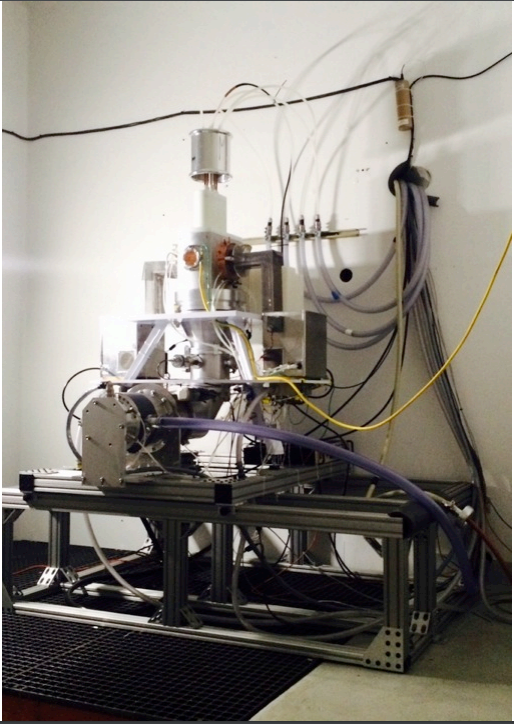
\includegraphics[width=\columnwidth]{./figures/Capture.PNG}
        \subfigimg[scale=0.47]{}{./figures/51Cr.pdf}
%         \caption{ Decay curve for the isomeric transition of \ce{^{115m}In}.}
         \refstepcounter{subfigure}\label{fig:51Cr}
    \end{subfigure}%
     \begin{subfigure}[t]{0.49\textwidth}
        \centering
%         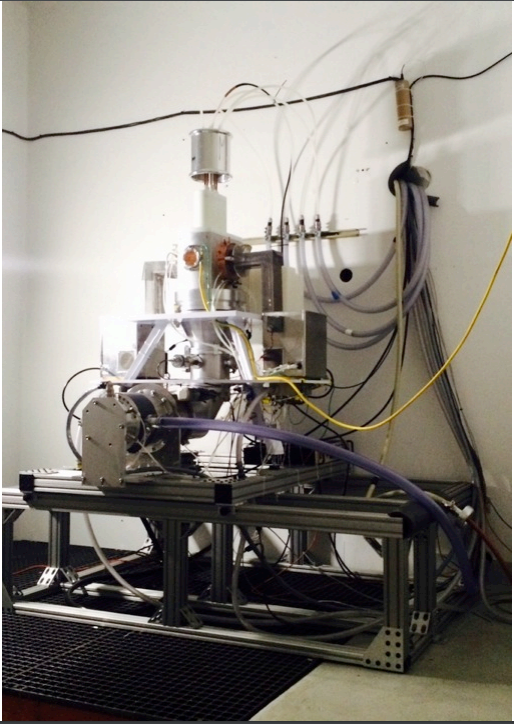
\includegraphics[width=\columnwidth]{./figures/Capture.PNG}
%         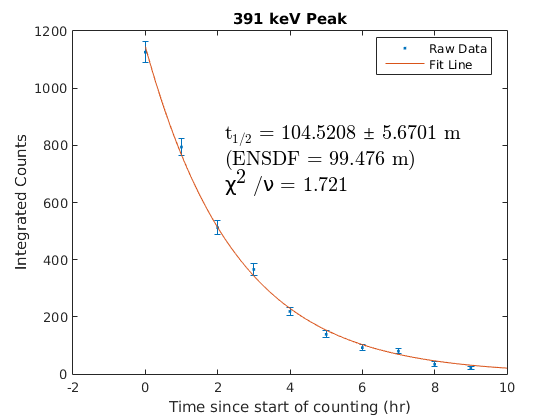
\includegraphics[scale=0.6]{./figures/391keV_curve2.png}
        \subfigimg[scale=0.465]{}{./figures/52gMn.pdf}
%         \caption{ Decay curve for the isomeric transition of \ce{^{113m}In}.}
         \refstepcounter{subfigure}\label{fig:52gMn}
    \end{subfigure}%
    \\
    \begin{subfigure}[t]{0.49\textwidth}
        \centering
%         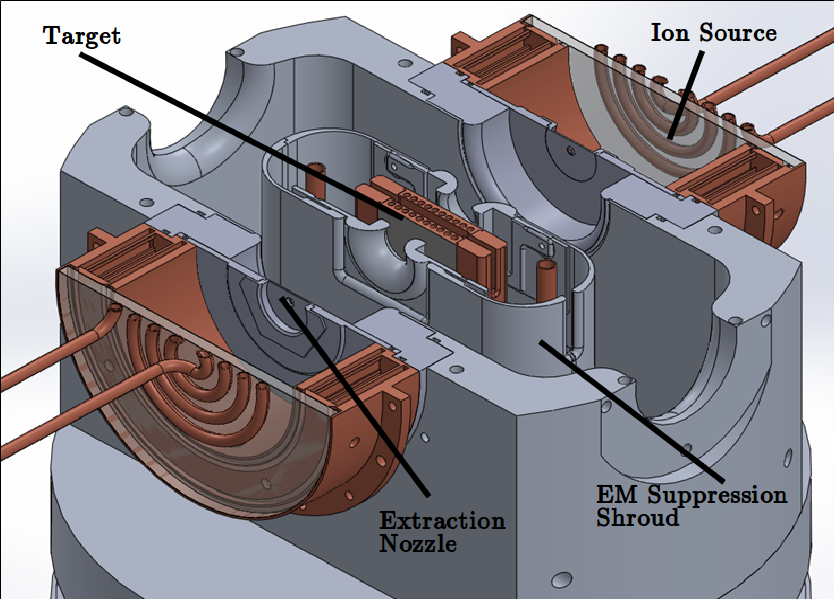
\includegraphics[width=\textwidth]{./figures/target2.png}
        \subfigimg[scale=0.47]{}{./figures/54Mn.pdf}
%         \caption{Decay curve for the $\beta^-$ decay of \ce{^{116}In}.}
                 \refstepcounter{subfigure}\label{fig:54Mn}
    \end{subfigure}
     \begin{subfigure}[t]{0.49\textwidth}
        \centering
%         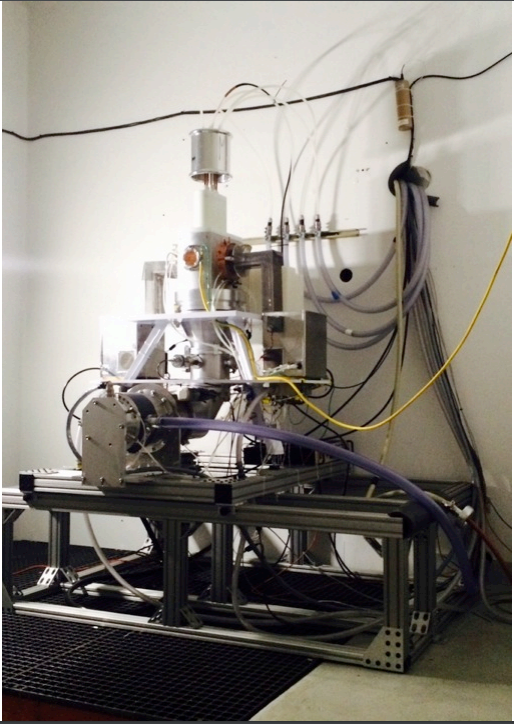
\includegraphics[width=\columnwidth]{./figures/Capture.PNG}
        \subfigimg[scale=0.47]{}{./figures/55Co.pdf}
%         \caption{ Decay curve for the $\beta^+$ decay of \ce{^{64}Cu}.}
        \refstepcounter{subfigure} \label{fig:55Co}
    \end{subfigure}%
    \\
    \begin{subfigure}[t]{0.49\textwidth}
        \centering
%         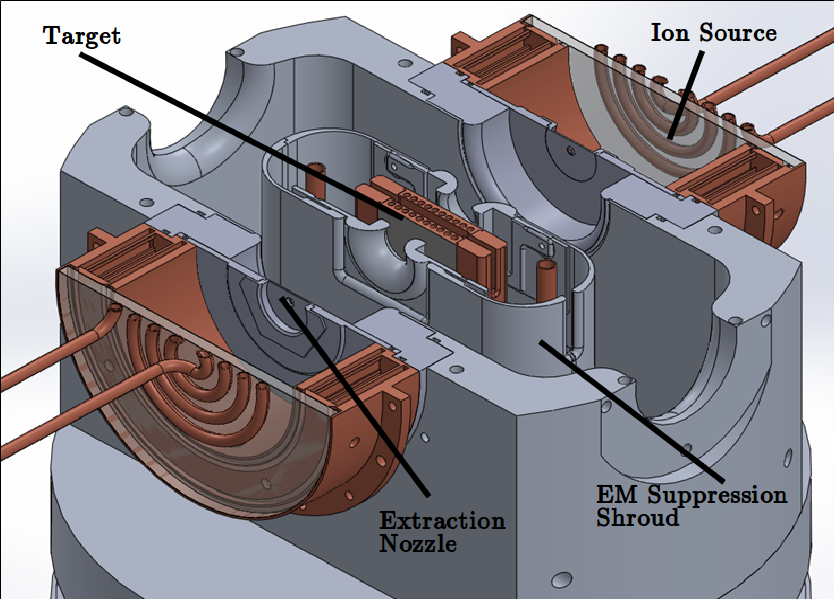
\includegraphics[width=\textwidth]{./figures/target2.png}
        \subfigimg[scale=0.465]{}{./figures/56Ni.pdf}
%         \caption{Decay curve for the $\beta^-$ decay of \ce{^{116}In}.}
                 \refstepcounter{subfigure}\label{fig:56Ni}
    \end{subfigure}
     \begin{subfigure}[t]{0.49\textwidth}
        \centering
%         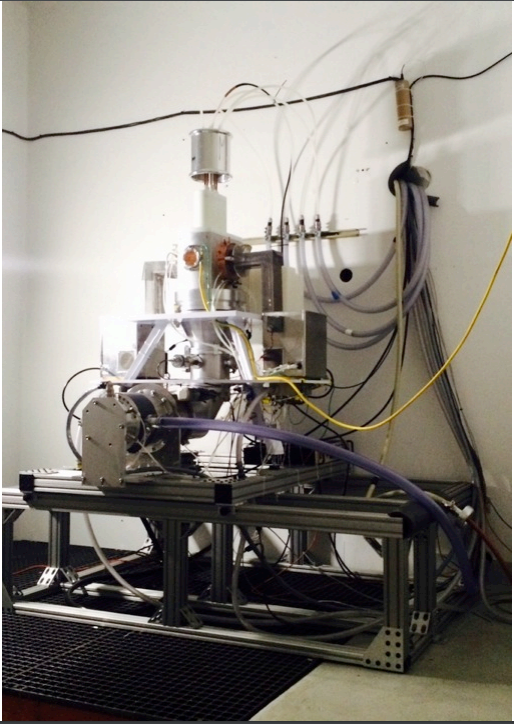
\includegraphics[width=\columnwidth]{./figures/Capture.PNG}
        \subfigimg[scale=0.47]{}{./figures/57Co.pdf}
%         \caption{ Decay curve for the $\beta^+$ decay of \ce{^{64}Cu}.}
        \refstepcounter{subfigure} \label{fig:57Co}
    \end{subfigure}%
%     \caption{Decay curves used to verify photopeak transition assignment. (a) Decay curve for the isomeric transition of \ce{^{115m}In}, (b) decay curve for the isomeric transition of \ce{^{113m}In}, (c) decay curve for the $\beta^-$ decay of \ce{^{116}In}, and (d) decay curve for the $\beta^+$ decay of \ce{^{64}Cu}.}
     \label{fig:xs_curves_p1}
\end{figure*}




\begin{figure*}
    \centering
    \begin{subfigure}[t]{0.49\textwidth}
        \centering
%         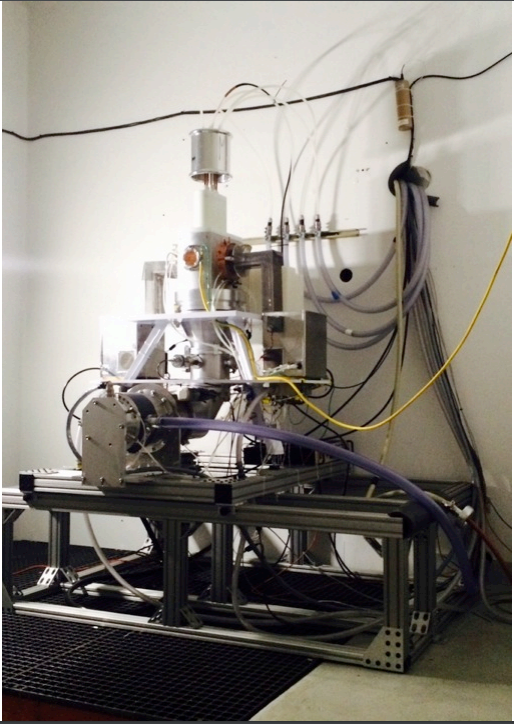
\includegraphics[width=\columnwidth]{./figures/Capture.PNG}
        \subfigimg[scale=0.47]{}{./figures/57Ni.pdf}
%         \caption{ Decay curve for the isomeric transition of \ce{^{115m}In}.}
         \refstepcounter{subfigure}\label{fig:57Ni}
    \end{subfigure}%
     \begin{subfigure}[t]{0.49\textwidth}
        \centering
%         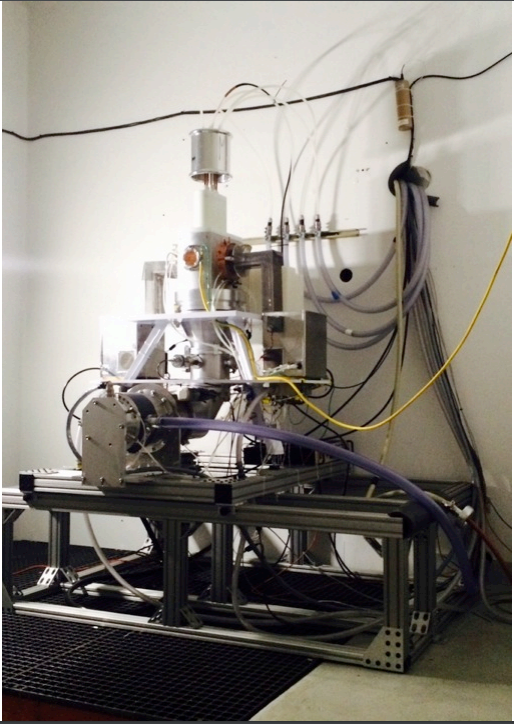
\includegraphics[width=\columnwidth]{./figures/Capture.PNG}
%         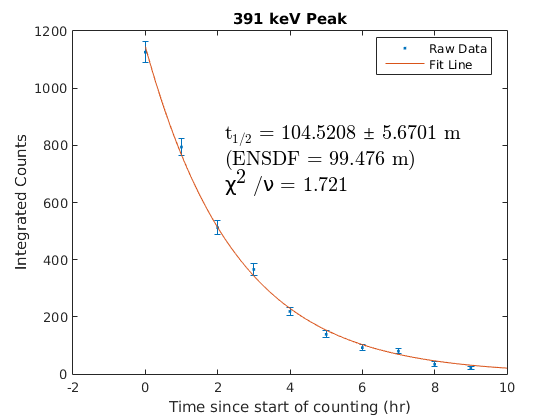
\includegraphics[scale=0.6]{./figures/391keV_curve2.png}
        \subfigimg[scale=0.47]{}{./figures/58Co.pdf}
%         \caption{ Decay curve for the isomeric transition of \ce{^{113m}In}.}
         \refstepcounter{subfigure}\label{fig:58Co}
    \end{subfigure}%
    \\
    \begin{subfigure}[t]{0.49\textwidth}
        \centering
%         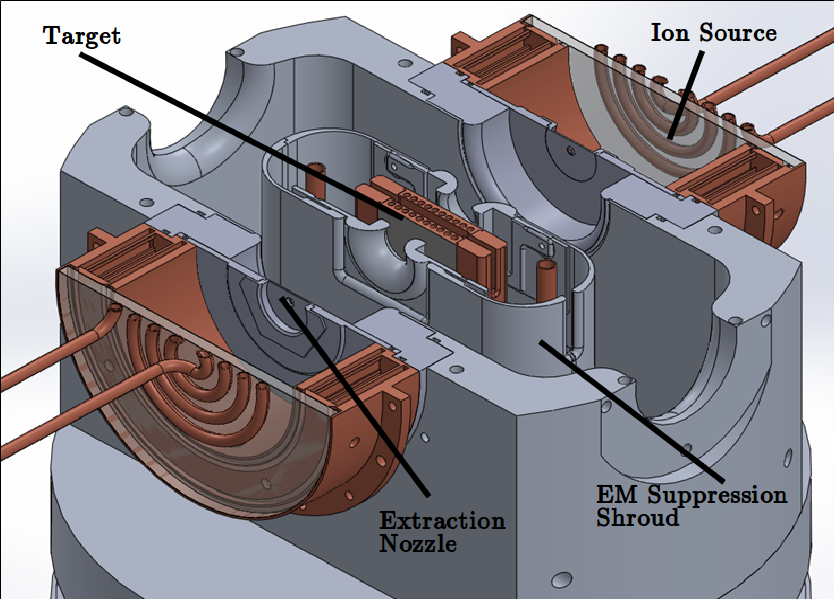
\includegraphics[width=\textwidth]{./figures/target2.png}
        \subfigimg[scale=0.465]{}{./figures/59Fe.pdf}
%         \caption{Decay curve for the $\beta^-$ decay of \ce{^{116}In}.}
                 \refstepcounter{subfigure}\label{fig:59Fe}
    \end{subfigure}
     \begin{subfigure}[t]{0.49\textwidth}
        \centering
%         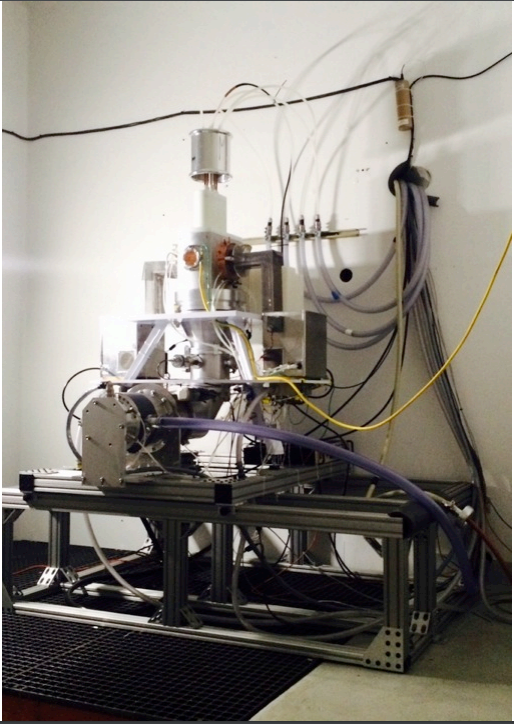
\includegraphics[width=\columnwidth]{./figures/Capture.PNG}
        \subfigimg[scale=0.47]{}{./figures/60Co.pdf}
%         \caption{ Decay curve for the $\beta^+$ decay of \ce{^{64}Cu}.}
        \refstepcounter{subfigure} \label{fig:60Co}
    \end{subfigure}%
    \\
    \begin{subfigure}[t]{0.49\textwidth}
        \centering
%         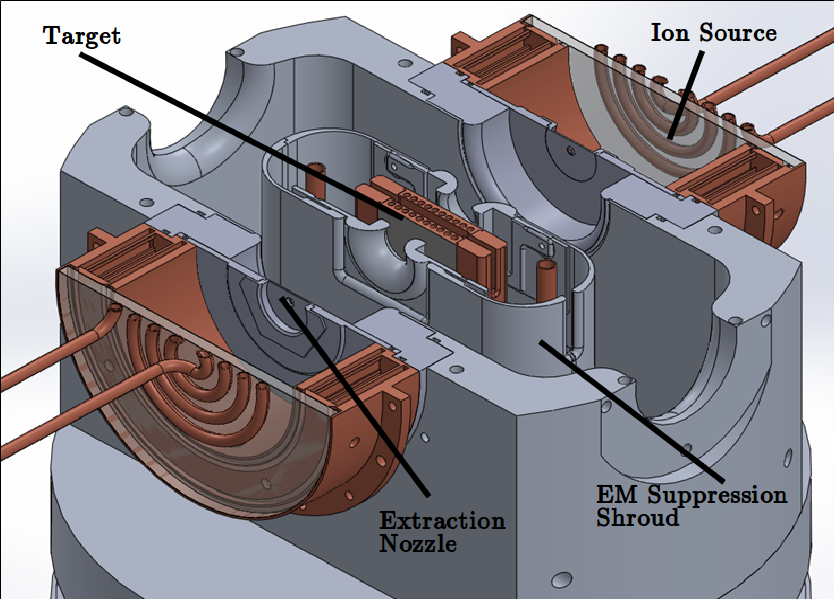
\includegraphics[width=\textwidth]{./figures/target2.png}
        \subfigimg[scale=0.47]{}{./figures/61Cu.pdf}
%         \caption{Decay curve for the $\beta^-$ decay of \ce{^{116}In}.}
                 \refstepcounter{subfigure}\label{fig:61Cu}
    \end{subfigure}
     \begin{subfigure}[t]{0.49\textwidth}
        \centering
%         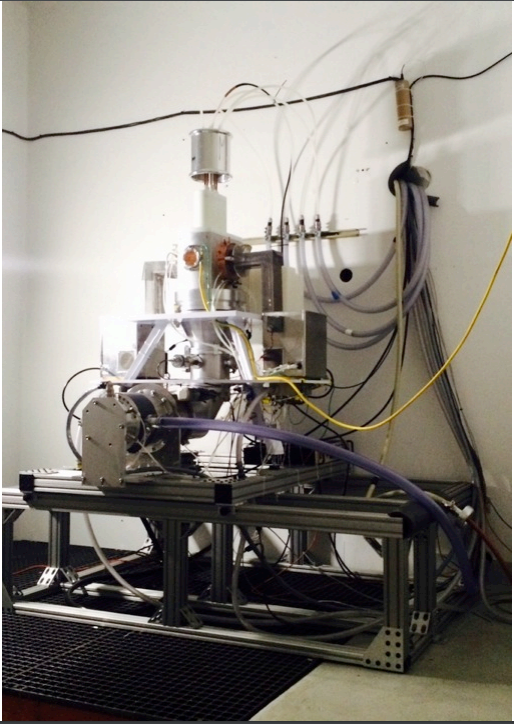
\includegraphics[width=\columnwidth]{./figures/Capture.PNG}
        \subfigimg[scale=0.47]{}{./figures/64Cu.pdf}
%         \caption{ Decay curve for the $\beta^+$ decay of \ce{^{64}Cu}.}
        \refstepcounter{subfigure} \label{fig:64Cu}
    \end{subfigure}%
%     \caption{Decay curves used to verify photopeak transition assignment. (a) Decay curve for the isomeric transition of \ce{^{115m}In}, (b) decay curve for the isomeric transition of \ce{^{113m}In}, (c) decay curve for the $\beta^-$ decay of \ce{^{116}In}, and (d) decay curve for the $\beta^+$ decay of \ce{^{64}Cu}.}
     \label{fig:xs_curves_p2}
\end{figure*}



\begin{figure*}
    \centering
    \begin{subfigure}[t]{0.49\textwidth}
        \centering
%         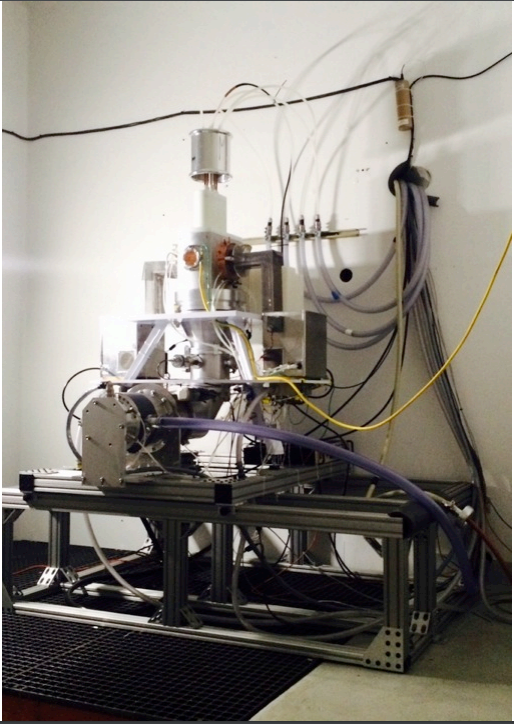
\includegraphics[width=\columnwidth]{./figures/Capture.PNG}
        \subfigimg[scale=0.47]{}{./figures/82mRb.pdf}
%         \caption{ Decay curve for the isomeric transition of \ce{^{115m}In}.}
         \refstepcounter{subfigure}\label{fig:82mRb}
    \end{subfigure}%
     \begin{subfigure}[t]{0.49\textwidth}
        \centering
%         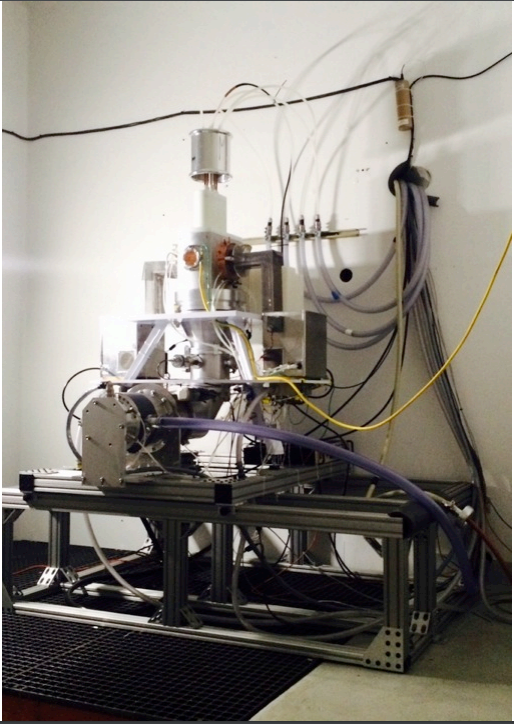
\includegraphics[width=\columnwidth]{./figures/Capture.PNG}
%         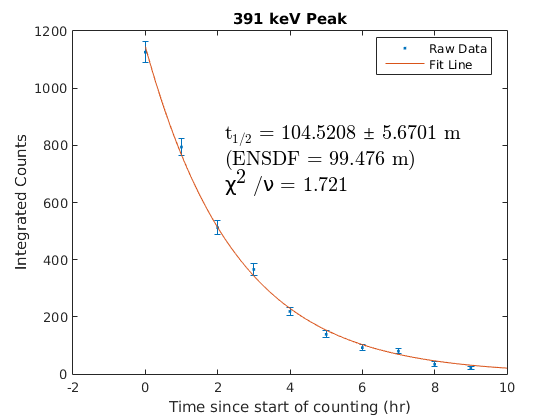
\includegraphics[scale=0.6]{./figures/391keV_curve2.png}
        \subfigimg[scale=0.47]{}{./figures/83Sr.pdf}
%         \caption{ Decay curve for the isomeric transition of \ce{^{113m}In}.}
         \refstepcounter{subfigure}\label{fig:83Sr}
    \end{subfigure}%
    \\
    \begin{subfigure}[t]{0.49\textwidth}
        \centering
%         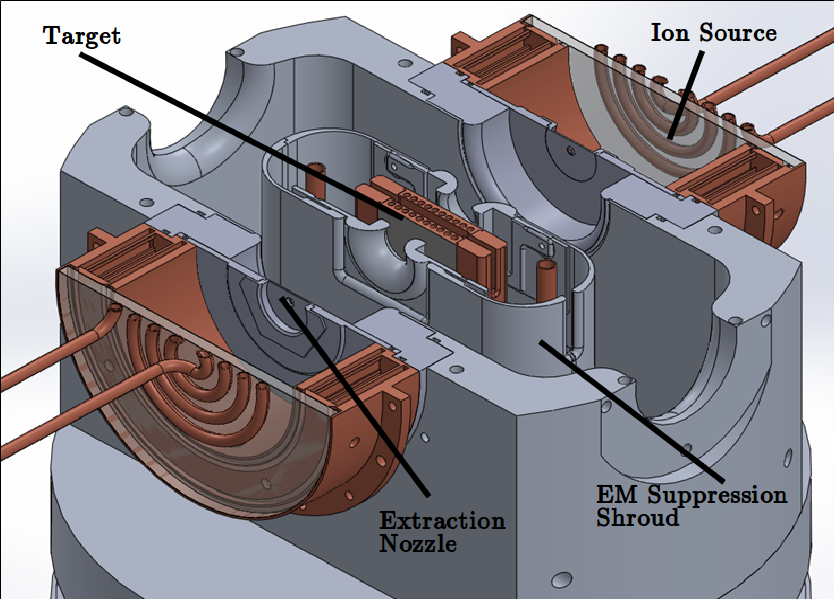
\includegraphics[width=\textwidth]{./figures/target2.png}
        \subfigimg[scale=0.47]{}{./figures/85Y.pdf}
%         \caption{Decay curve for the $\beta^-$ decay of \ce{^{116}In}.}
                 \refstepcounter{subfigure}\label{fig:85Y}
    \end{subfigure}
     \begin{subfigure}[t]{0.49\textwidth}
        \centering
%         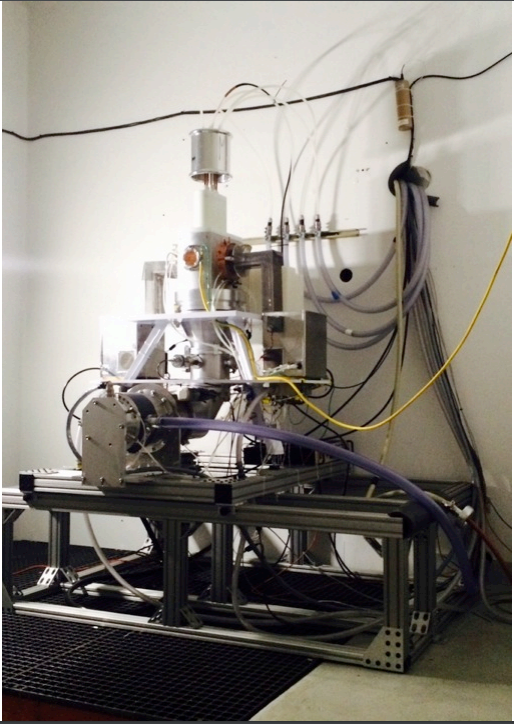
\includegraphics[width=\columnwidth]{./figures/Capture.PNG}
        \subfigimg[scale=0.47]{}{./figures/86Y.pdf}
%         \caption{ Decay curve for the $\beta^+$ decay of \ce{^{64}Cu}.}
        \refstepcounter{subfigure} \label{fig:86Y}
    \end{subfigure}%
    \\
    \begin{subfigure}[t]{0.49\textwidth}
        \centering
%         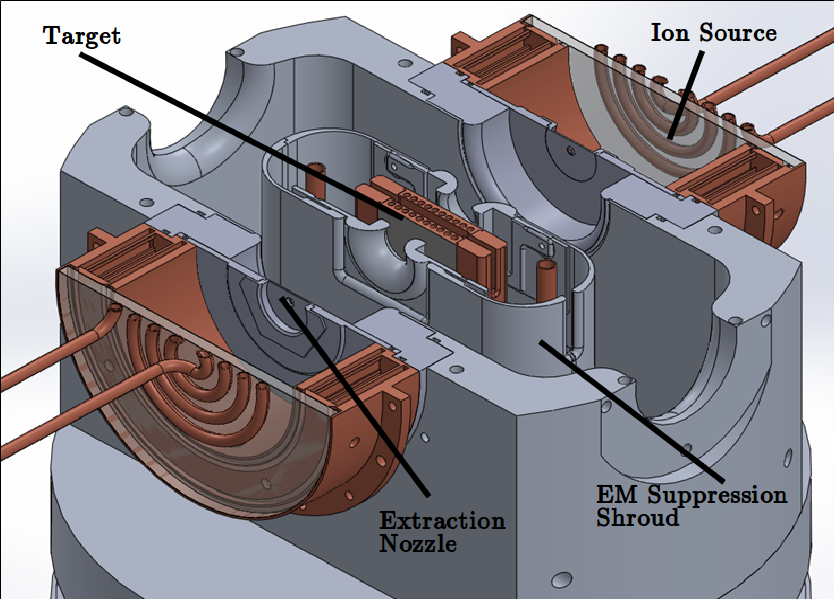
\includegraphics[width=\textwidth]{./figures/target2.png}
        \subfigimg[scale=0.47]{}{./figures/86Zr.pdf}
%         \caption{Decay curve for the $\beta^-$ decay of \ce{^{116}In}.}
                 \refstepcounter{subfigure}\label{fig:86Zr}
    \end{subfigure}
     \begin{subfigure}[t]{0.49\textwidth}
        \centering
%         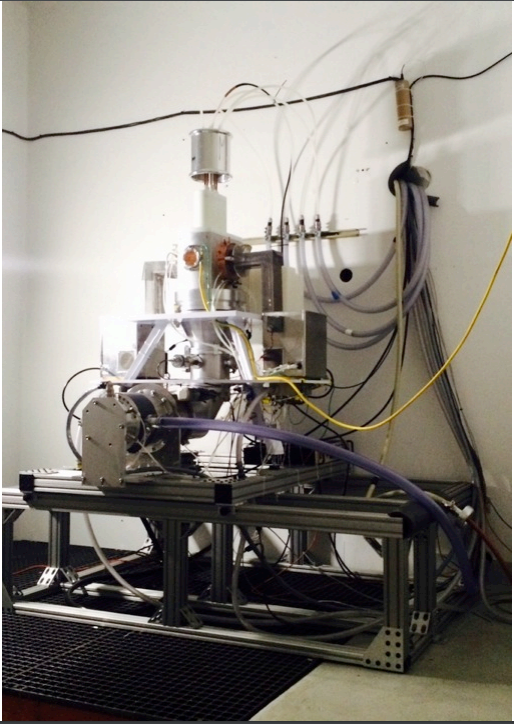
\includegraphics[width=\columnwidth]{./figures/Capture.PNG}
        \subfigimg[scale=0.47]{}{./figures/87Y.pdf}
%         \caption{ Decay curve for the $\beta^+$ decay of \ce{^{64}Cu}.}
        \refstepcounter{subfigure} \label{fig:87Y}
    \end{subfigure}%
%     \caption{Decay curves used to verify photopeak transition assignment. (a) Decay curve for the isomeric transition of \ce{^{115m}In}, (b) decay curve for the isomeric transition of \ce{^{113m}In}, (c) decay curve for the $\beta^-$ decay of \ce{^{116}In}, and (d) decay curve for the $\beta^+$ decay of \ce{^{64}Cu}.}
     \label{fig:xs_curves_p3}
\end{figure*}



\begin{figure*}
    \centering
    \begin{subfigure}[t]{0.49\textwidth}
        \centering
%         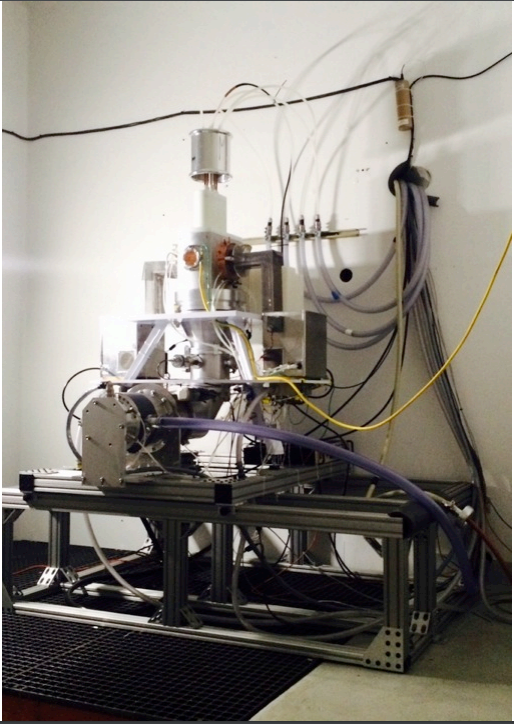
\includegraphics[width=\columnwidth]{./figures/Capture.PNG}
        \subfigimg[scale=0.47]{}{./figures/87Zr.pdf}
%         \caption{ Decay curve for the isomeric transition of \ce{^{115m}In}.}
         \refstepcounter{subfigure}\label{fig:87Zr}
    \end{subfigure}%
     \begin{subfigure}[t]{0.49\textwidth}
        \centering
%         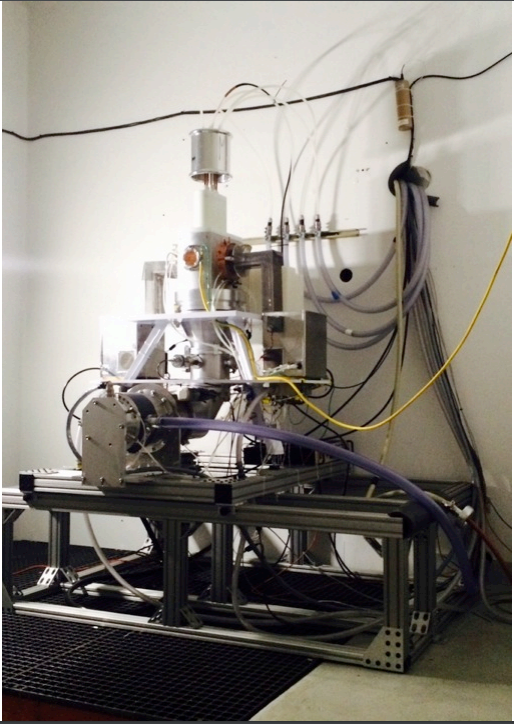
\includegraphics[width=\columnwidth]{./figures/Capture.PNG}
%         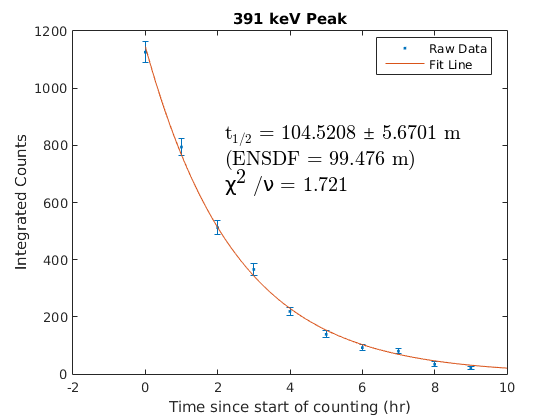
\includegraphics[scale=0.6]{./figures/391keV_curve2.png}
        \subfigimg[scale=0.47]{}{./figures/88Y.pdf}
%         \caption{ Decay curve for the isomeric transition of \ce{^{113m}In}.}
         \refstepcounter{subfigure}\label{fig:88Y}
    \end{subfigure}%
    \\
    \begin{subfigure}[t]{0.49\textwidth}
        \centering
%         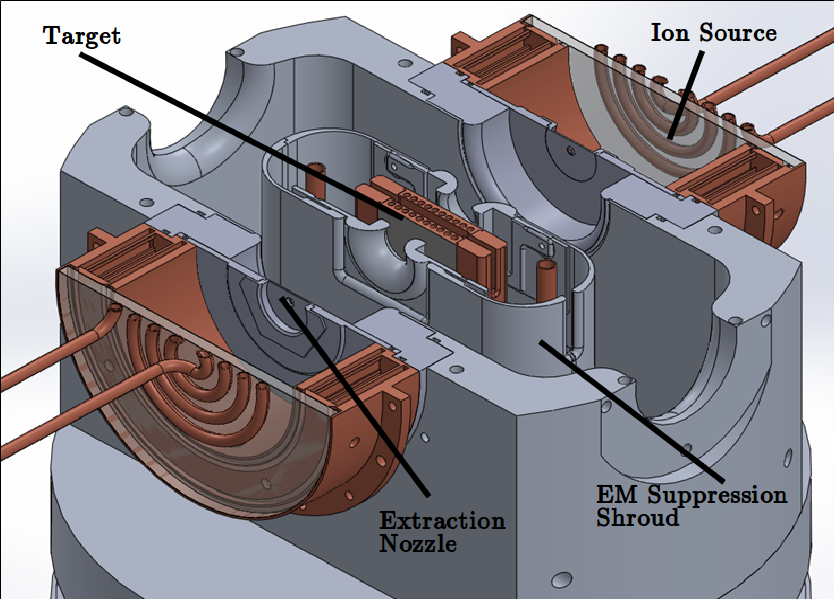
\includegraphics[width=\textwidth]{./figures/target2.png}
        \subfigimg[scale=0.47]{}{./figures/88Zr.pdf}
%         \caption{Decay curve for the $\beta^-$ decay of \ce{^{116}In}.}
                 \refstepcounter{subfigure}\label{fig:88Zr}
    \end{subfigure}
     \begin{subfigure}[t]{0.49\textwidth}
        \centering
%         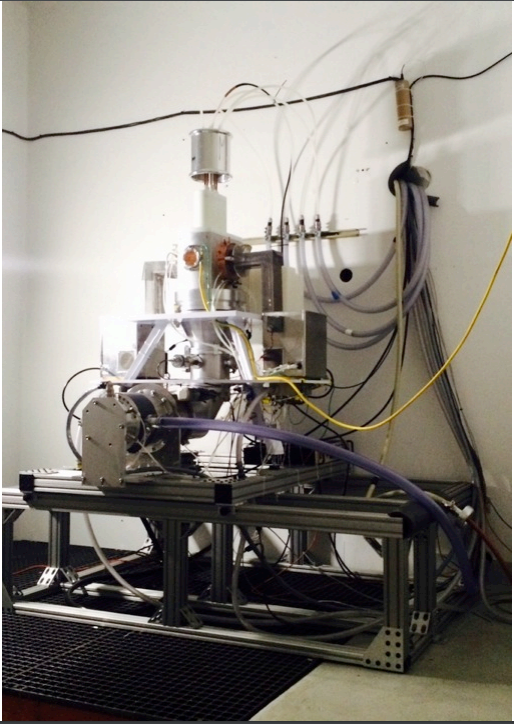
\includegraphics[width=\columnwidth]{./figures/Capture.PNG}
        \subfigimg[scale=0.47]{}{./figures/89Nb.pdf}
%         \caption{ Decay curve for the $\beta^+$ decay of \ce{^{64}Cu}.}
        \refstepcounter{subfigure} \label{fig:89Nb}
    \end{subfigure}%
    \\
    \begin{subfigure}[t]{0.49\textwidth}
        \centering
%         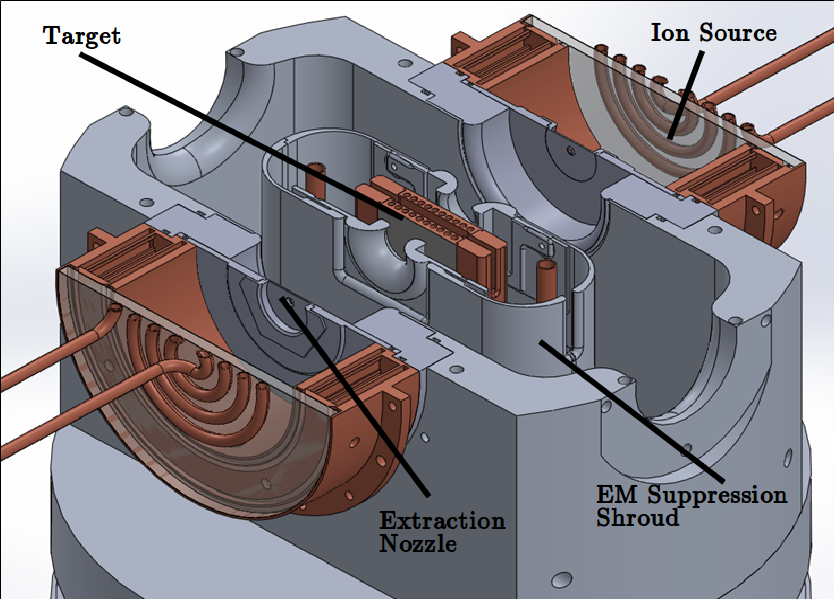
\includegraphics[width=\textwidth]{./figures/target2.png}
        \subfigimg[scale=0.47]{}{./figures/89Zr.pdf}
%         \caption{Decay curve for the $\beta^-$ decay of \ce{^{116}In}.}
                 \refstepcounter{subfigure}\label{fig:89Zr}
    \end{subfigure}
     \begin{subfigure}[t]{0.49\textwidth}
        \centering
%         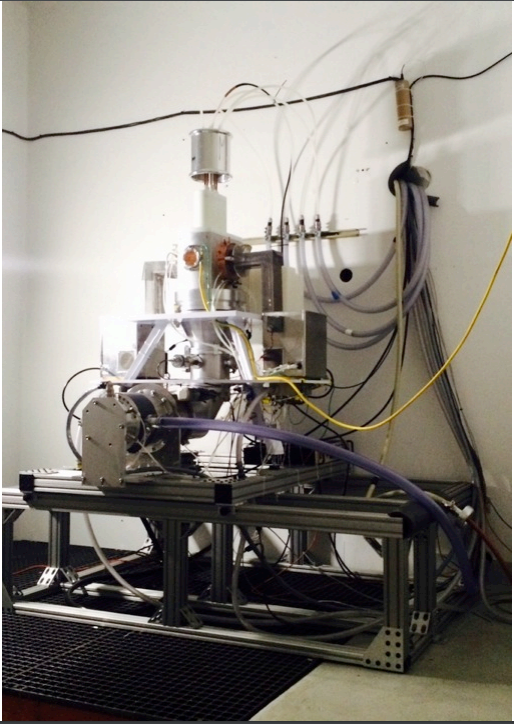
\includegraphics[width=\columnwidth]{./figures/Capture.PNG}
        \subfigimg[scale=0.465]{}{./figures/90Mo.pdf}
%         \caption{ Decay curve for the $\beta^+$ decay of \ce{^{64}Cu}.}
        \refstepcounter{subfigure} \label{fig:90Mo}
    \end{subfigure}%
%     \caption{Decay curves used to verify photopeak transition assignment. (a) Decay curve for the isomeric transition of \ce{^{115m}In}, (b) decay curve for the isomeric transition of \ce{^{113m}In}, (c) decay curve for the $\beta^-$ decay of \ce{^{116}In}, and (d) decay curve for the $\beta^+$ decay of \ce{^{64}Cu}.}
     \label{fig:xs_curves_p4}
\end{figure*}




\begin{figure*}
    \centering
    \begin{subfigure}[t]{0.49\textwidth}
        \centering
%         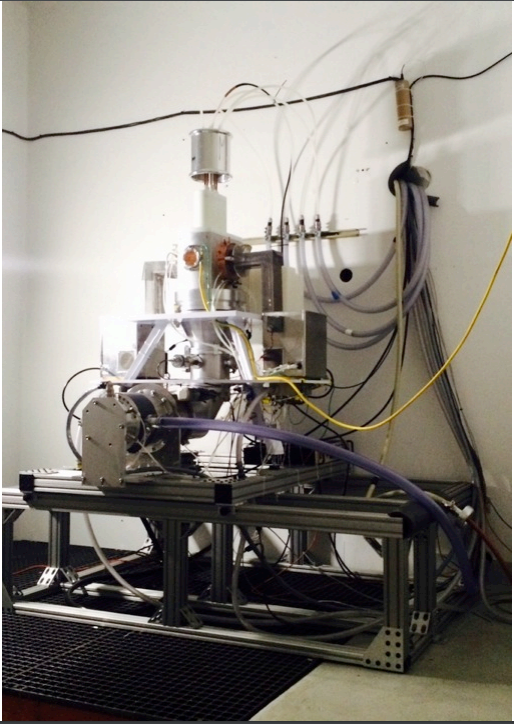
\includegraphics[width=\columnwidth]{./figures/Capture.PNG}
        \subfigimg[scale=0.47]{}{./figures/90Nb.pdf}
%         \caption{ Decay curve for the isomeric transition of \ce{^{115m}In}.}
         \refstepcounter{subfigure}\label{fig:90Nb}
    \end{subfigure}%
     \begin{subfigure}[t]{0.49\textwidth}
        \centering
%         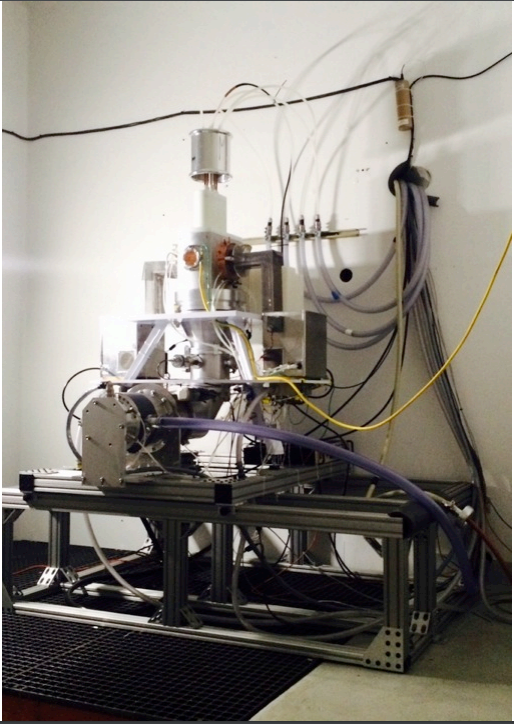
\includegraphics[width=\columnwidth]{./figures/Capture.PNG}
%         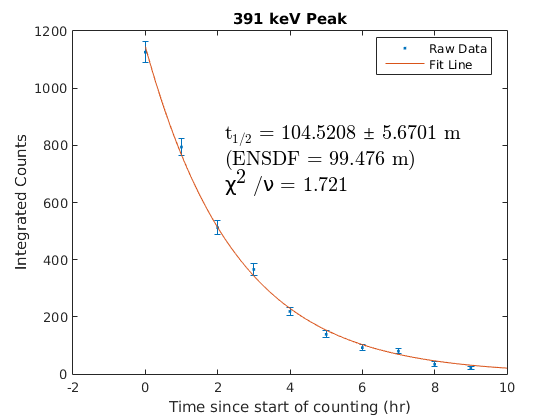
\includegraphics[scale=0.6]{./figures/391keV_curve2.png}
        \subfigimg[scale=0.47]{}{./figures/91mNb.pdf}
%         \caption{ Decay curve for the isomeric transition of \ce{^{113m}In}.}
         \refstepcounter{subfigure}\label{fig:91mNb}
    \end{subfigure}%
    \\
    \begin{subfigure}[t]{0.49\textwidth}
        \centering
%         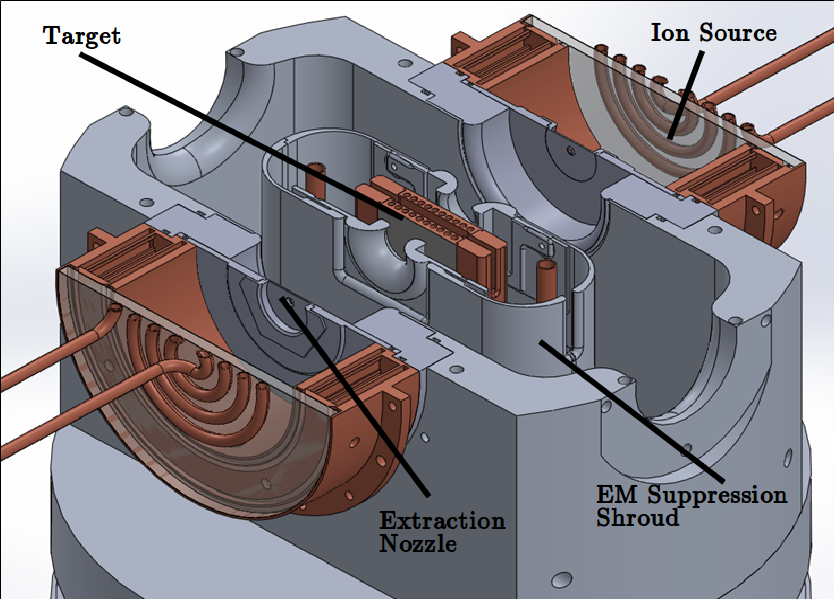
\includegraphics[width=\textwidth]{./figures/target2.png}
        \subfigimg[scale=0.47]{}{./figures/92mNb.pdf}
%         \caption{Decay curve for the $\beta^-$ decay of \ce{^{116}In}.}
                 \refstepcounter{subfigure}\label{fig:92mNb}
    \end{subfigure}
     \begin{subfigure}[t]{0.49\textwidth}
        \centering
%         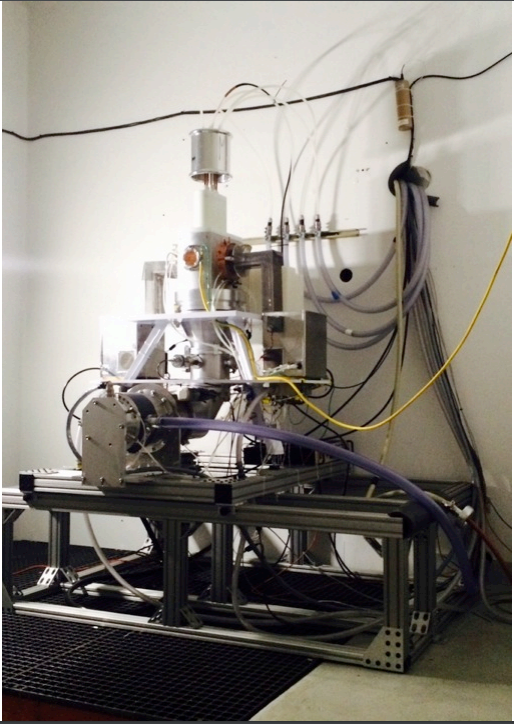
\includegraphics[width=\columnwidth]{./figures/Capture.PNG}
        \subfigimg[scale=0.47]{}{./figures/93mMo.pdf}
%         \caption{ Decay curve for the $\beta^+$ decay of \ce{^{64}Cu}.}
        \refstepcounter{subfigure} \label{fig:93mMo}
    \end{subfigure}%
%     \caption{Decay curves used to verify photopeak transition assignment. (a) Decay curve for the isomeric transition of \ce{^{115m}In}, (b) decay curve for the isomeric transition of \ce{^{113m}In}, (c) decay curve for the $\beta^-$ decay of \ce{^{116}In}, and (d) decay curve for the $\beta^+$ decay of \ce{^{64}Cu}.}
     \label{fig:xs_curves_p5}
\end{figure*}




% 
% 
\section{Measured isomer-to-ground state branching ratios } \label{ibr_figures}

Plots of the isomer-to-ground state ratios measured in this work are presented here, in comparison with literature data and reaction modeling codes \cite{MICHEL1997153,Ditroi2008,Titarenko2011,Graves2016}.





\begin{figure*}
    \centering
    \begin{subfigure}[t]{0.49\textwidth}
        \centering
%         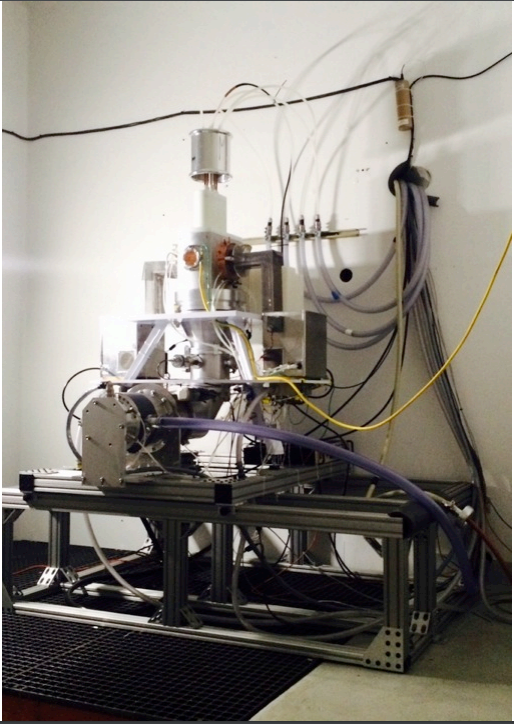
\includegraphics[width=\columnwidth]{./figures/Capture.PNG}
        \subfigimg[scale=0.47]{}{./figures/52Mn_IBR.pdf}
%         \caption{ Decay curve for the isomeric transition of \ce{^{115m}In}.}
         \refstepcounter{subfigure}\label{fig:52Mn_IBR}
    \end{subfigure}%
     \begin{subfigure}[t]{0.49\textwidth}
        \centering
%         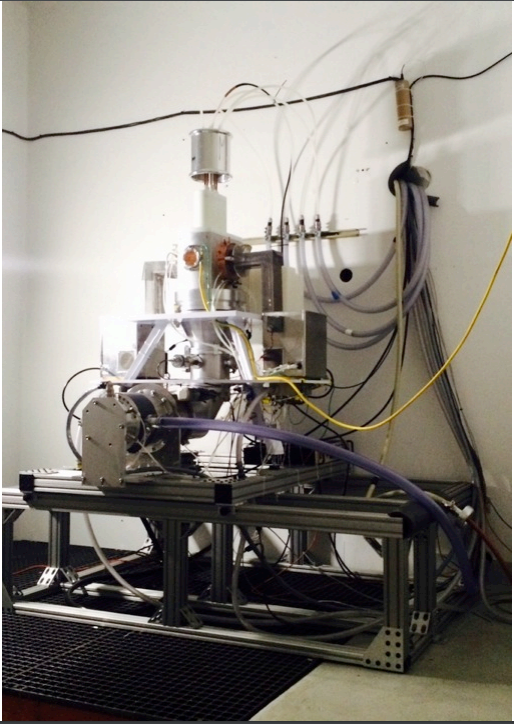
\includegraphics[width=\columnwidth]{./figures/Capture.PNG}
%         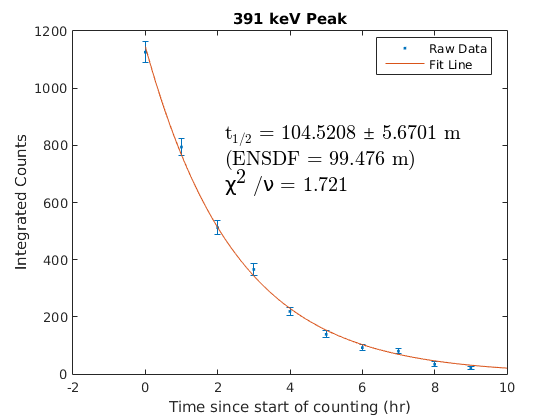
\includegraphics[scale=0.6]{./figures/391keV_curve2.png}
        \subfigimg[scale=0.47]{}{./figures/58Co_IBR.pdf}
%         \caption{ Decay curve for the isomeric transition of \ce{^{113m}In}.}
         \refstepcounter{subfigure}\label{fig:58Co_IBR}
    \end{subfigure}%
    \\
    \begin{subfigure}[t]{0.49\textwidth}
        \centering
%         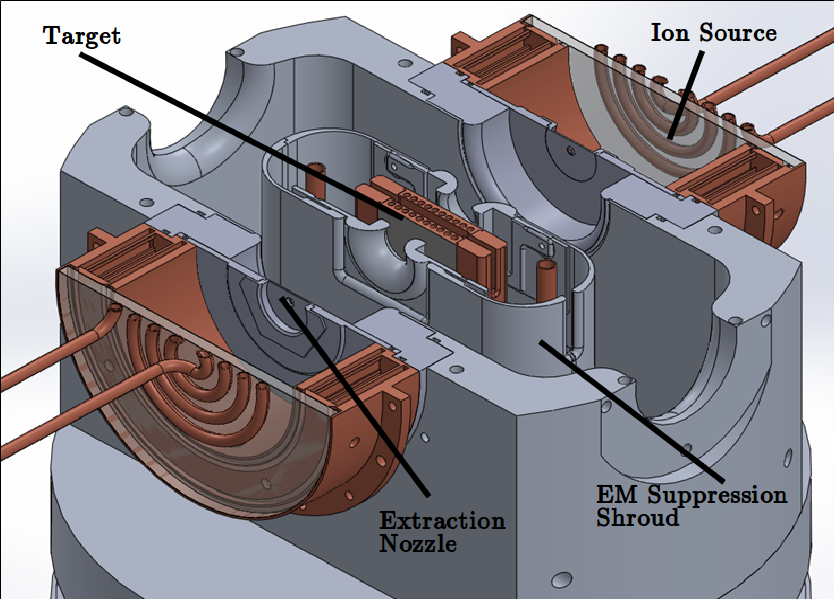
\includegraphics[width=\textwidth]{./figures/target2.png}
        \subfigimg[scale=0.47]{}{./figures/85Y_IBR.pdf}
%         \caption{Decay curve for the $\beta^-$ decay of \ce{^{116}In}.}
                 \refstepcounter{subfigure}\label{fig:85Y_IBR}
    \end{subfigure}
     \begin{subfigure}[t]{0.49\textwidth}
        \centering
%         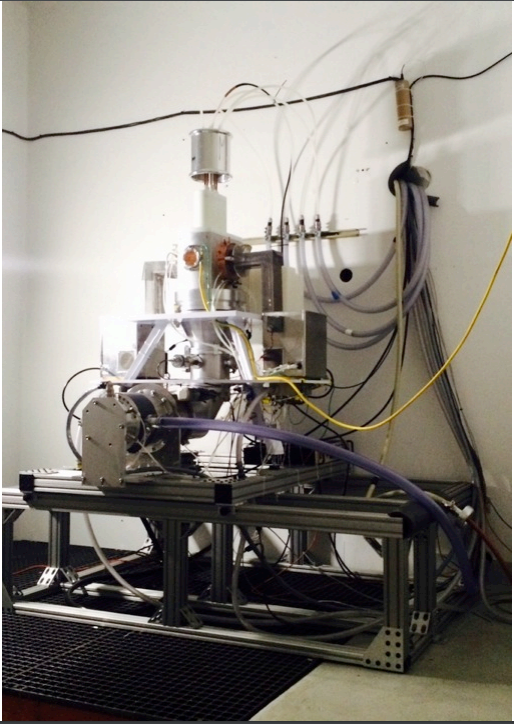
\includegraphics[width=\columnwidth]{./figures/Capture.PNG}
        \subfigimg[scale=0.47]{}{./figures/87Y_IBR.pdf}
%         \caption{ Decay curve for the $\beta^+$ decay of \ce{^{64}Cu}.}
        \refstepcounter{subfigure} \label{fig:87Y_IBR}
    \end{subfigure}%
    \\
    \begin{subfigure}[t]{0.49\textwidth}
        \centering
%         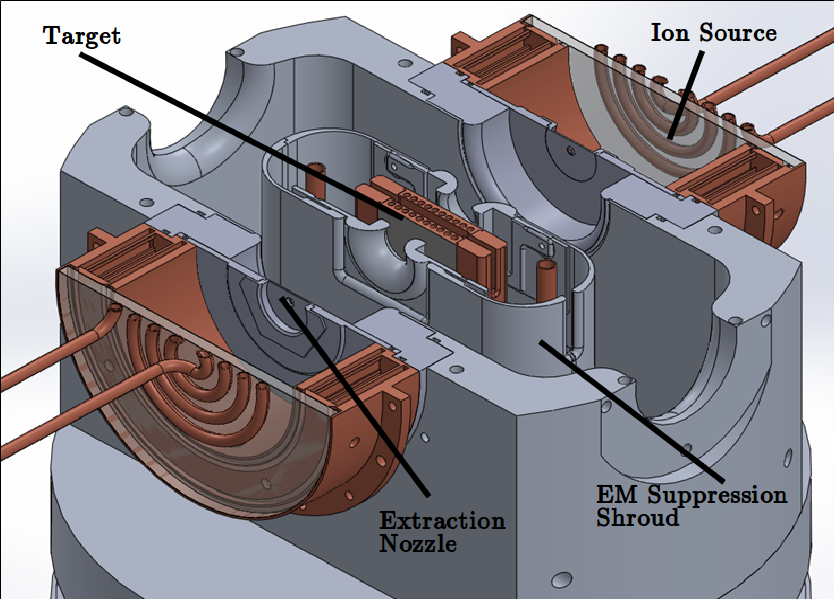
\includegraphics[width=\textwidth]{./figures/target2.png}
        \subfigimg[scale=0.47]{}{./figures/89Nb_IBR.pdf}
%         \caption{Decay curve for the $\beta^-$ decay of \ce{^{116}In}.}
                 \refstepcounter{subfigure}\label{fig:89Nb_IBR}
    \end{subfigure}
     \label{fig:ibr_curves}
\end{figure*}


% 
% 
% % \begin{figure}[h]
% %  \centering
% %  \includegraphics[scale=0.7]{./hw04/fit110Ru240-cropped.pdf}
% %  % fit110Ru240.ps: 570x750 pixel, 72dpi, 20.11x26.46 cm, bb=0 0 570 750
% %  \caption{Fit to the \ce{^{110}Ru} 240.7 keV peak and its surroundings.}
% %  \label{fig:110Ru240}
% % \end{figure}
% % 

% \twocolumn

%% References with BibTeX database:

% \bibliographystyle{elsarticle-num}
% \bibliographystyle{elsarticle-harv}
% \bibliographystyle{elsarticle-num-names}
% \bibliography{<your-bib-database>}
% \addcontentsline{toc}{chapter}{Bibliography}
\bibliographystyle{elsarticle-num}
% \bibliographystyle{ieeetr}
\bibliography{../../library}
% \thispagestyle{fancyTOC}




%% Authors are advised to use a BibTeX database file for their reference list.
%% The provided style file elsarticle-num.bst formats references in the required Procedia style

%% For references without a BibTeX database:

% \begin{thebibliography}{00}

%% \bibitem must have the following form:
%%   \bibitem{key}...
%% 

% \bibitem{}

% \end{thebibliography}

\end{document}

%%
%% End of file `ecrc-template.tex'. 